%*******************************************************************************
%****************************** Sixth Chapter *********************************
%*******************************************************************************

\chapter{ns-3 Implementation of LISP and LISP-MN}
\label{cha:ns-3}

% **************************** Define Graphics Path **************************
\ifpdf
    \graphicspath{{Chapter7/Pics/Raster/}{Chapter7/Pics/PDF/}{Chapter7/}}
\else
    \graphicspath{{Chapter7/Pics/Vector/}{Chapter7/}}
\fi

%-< ABSTRACT >--------------------------------------------------------------------
The \emph{Locator/Identifier Separation Protocol} (LISP) reconstructs the current IP addressing space to improve the scalability and no interrupt mobility issues. LISP Mobile Node (LISP-MN) is based on the basic LISP functionality to provide seamless mobility across networks. The basic LISP architecture is deployed on LISP Beta Network and LISP-Lab platform to offer the researchers a realistic experimental environment, but both do not support LISP-MN. Some simulation models with LISP extensions are implemented on various simulators, but are unfortunately not open source. Providing a free and flexible simulation model with the basic LISP architecture as well as the extensions so to help researchers quickly test new LISP behaviors motivates our work. This paper introduces the implementation of the basic LISP architecture model and LISP-MN on the simulator ns-3. It also provides the evaluation results in mobility scenario to validate the model and shows when the current proposal of LISP-MN is behind a LISP-site has a very high delay during the handover procedure.

The rest of chapter is organized as follows: Sec.~\ref{sec:ns3_intro} reviews LISP architecture, highlighting the LISP mobility mechanism; Sec.~\ref{sec:ns3_related_work} ... Sec.~\ref{sec:ns3_modify} analyzes the design and implementation of our prototype, and afterwards, Sec.~\ref{sec:evaluation} presents preliminary evaluation results of our implementations. We finish with a discussion and some ideas for future work.
%-< ABSTRACT >--------------------------------------------------------------------

\section{Introduction}
\label{sec:ns3_intro}
% The research community are on the need of an open source LISP/LISP-MN simulator to facilitate the LISP-related studies. There exist some research efforts to fulfill this gap, however these simulators are not available for the pubic neither covering LISP-MN. That's the motivation of this work and importance of our work.
% \begin{itemize}
%     \item present the shortcomings of measurements on the real Internet and thus the advantages of simulation
%     \item xx
% \end{itemize}
The \emph{Locator/Identifier Separation Protocol} (LISP)~\cite{rfc6830} is initially proposed to solve the scalability and flexibility issues of current Internet architecture, since it decouples the Routing Locators (RLOCs) and Endpoint Identifiers (EIDs). This allows that the BGP routing tables in Internet core just announce the globally routable RLOCs whereas EIDs are only locally used within the subnets. LISP is under standardization at the IETF around ten years and as it develops, more advantages are found, such as: seamless mobility at terminal or in the Data Center, IPv6 transition and traffic engineering~\cite{saucez2016locator}. Among them, the continuous communication without interruption during the handover of terminals becomes a hot topic recently.

To test the various features of LISP, two LISP testbeds are built: LISP Beta Network and LISP-Lab platform. But both of them are only the basic LISP architectures and do not support mobility functionality. Some platform-specific LISP implementations, such as: OpenLISP~\cite{phung2014openlisp}, Open Overlay Router (OOR)~\cite{LISPmob} and Cisco's implementation~\cite{CiscoIOS}, can provide realistic LISP evaluations but lack the flexibility to test the new features. A LISP simulator is a good choice for the researchers. To the best knowledge, LISP is first implemented on ns-3~\cite{ns3}, which is widely used by academic researchers and educational use in~\cite{lezama2009implementation}, but mobility support is not included as well. While within OMNET++ platform, LISP and mobility features are implemented~\cite{klein2012integration}. However, their source code is not available online. To promote the development of LISP and as ns-3 gradually shows the potential to take the momentum in network simulator domain~\cite{rana2017implementation}, it highlights the importance to implement LISP and its mobility extensions under ns-3 and motivates our work.

In this paper, we introduce the implementation of basic LISP functions and mobility features on ns-3 by both modifying the existent ns-3 modules and integrating the new modules. Our simulator is validated by achieving a mobility scenario, in which a terminal changes the attachment points by keeping the communication with the remote node. All the handover procedures are transparent to the terminal, however, the delay to receive the packets again presents high.

\section{Related work}
\label{sec:ns3_related_work}
%-< SUB SECTION >--------------------------------------------------------------------
% \subsection{Description of ns-3}
% \label{sec:descriptionns-3}
 ns-3~\cite{ns3} is a popular and free discrete-event network simulator for networking research. To be closer to the real implementation (in a real Operating System), easily include C-based implementation codes, ease debugging and reduce the cost on maintaining in a long term, C++ is prioritized to be the unique programming language for ns-3. Besides, ns-3 offers the possibility to visualize the simulation instance so to allow the users to visually confirm the packets flow as they expect.
%\begin{itemize}
%    \item Description of ns-3.
%    \item The simulator supporting LISP is introduced in Sec.~\ref{subsec:implementation_OMNet}.
%\end{itemize}


%%-< SECTION >--------------------------------------------------------------------
%\section{Simulation model}
%\label{sec:sim_model}


%-< SECTION >--------------------------------------------------------------------
\section{LISP/LISP-MN Implementation based on ns3}
\label{sec:ns3_modify}
It should be noted that this work is based on a prior implementation work by Lionel. However, his implementation has no support for LISP MN.

%-< FIGURE >--------------------------------------------------------------------
\begin{figure*}[!t]
	\centering
	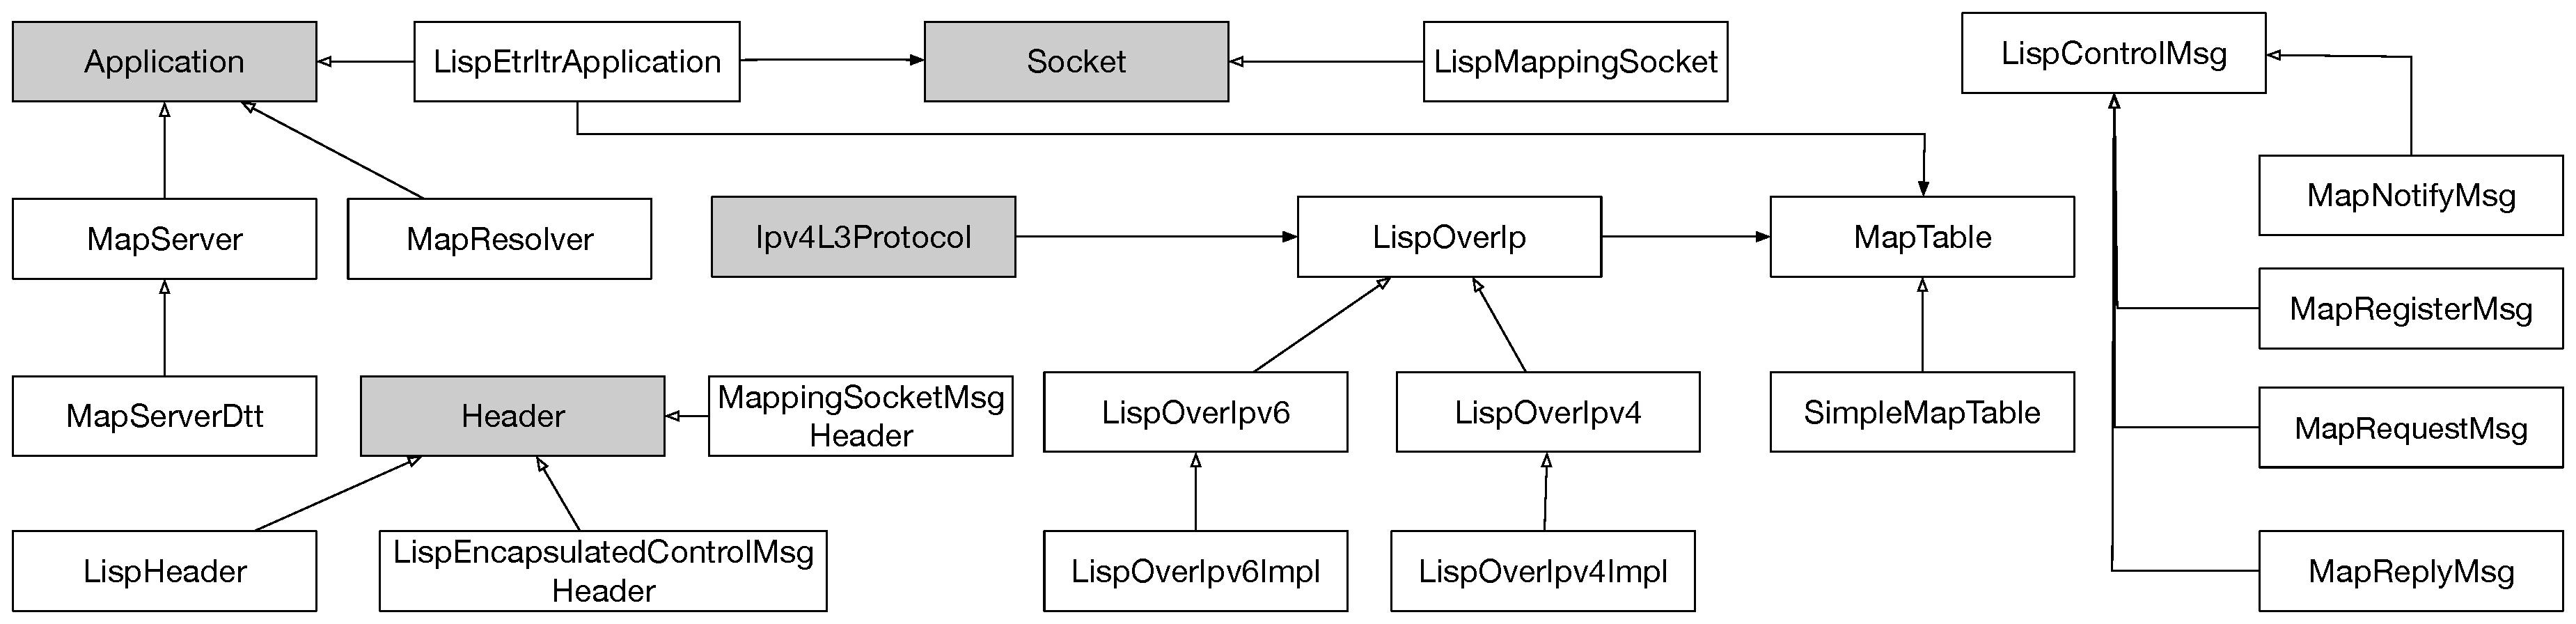
\includegraphics[width=\textwidth]{Pics/LISP-NS3-UML}
	\caption{UML diagram of LISP/LISP-MN implementation. The solid arrow refers to a composition relation, while the blank one refers to a inheritance relation.}
	\label{LISP-UML}
\end{figure*}
%-< END FIGURE >--------------------------------------------------------------------
Our implementation is under ns-3.26 and based on LISP~\cite{ietf-lisp-rfc6830bis-03} and LISP-MN standards~\cite{meyer-lisp-mn-16}. The main classes are shown in Fig.~\ref{LISP-UML} in form of UML diagram. The blank blocks refer to the classes that we added into ns-3, while darker blocks are classes already in ns-3. As a design choice, we implement LISP/LISP-MN functionalities by modifying and extending the \emph{internet} module of ns-3, instead of creating a new independent module. The justification of this design is that LISP/LISP-MN and legacy internet module have an interdependent relationship. However, this kind mutually dependent relationship between modules is not supported by ns-3. Inspired from design of OpenLISP~\cite{saucez2009openlisp}, the Data Plane implementation is in "kernel space" (i.e. ns-3's \emph{TCP/IP stack}) and Control Plane is implemented in "user space" (i.e. ns-3 \emph{Application}). The communication between LISP Data and Control Plane is developed via a dedicated socket (i.e. \emph{LispMappingSocket}) that inherits from ns-3 \emph{Socket} class. It should be noted that our implementation only supports IPv4 at time of this writing. The IPv6 support (i.e. the implementation related to IPv6 such as \emph{LispOverIpv6Impl}) is still in process.  

%-< SUB SECTION >--------------------------------------------------------------------
\subsection{Implementation of LISP Data Plane}
\label{subsec:modifyInternet}
%\begin{itemize}
%    \item Modification of Receive method
%    \item Modification of Delivery method
%    \item Implementation of LISP encapsulation and decapsulation
%\end{itemize}
A LISP-compatible node (terminal or router) should be capable of determining whether a packet should be passed to LISP-related procedure and retrieving the associated mapping information if necessary. To this end, a new class called \emph{LispOverIp} and its extended classes (refer to Fig.~\ref{LISP-UML}) are added to ns-3 \emph{internet} module. This class is in charge of checking whether necessary to do LISP-related operations (\emph{NeedEncapsulation()}, \emph{NeedDecapsulation()}), and encapsulating conventional IP packets (i.e., \emph{LispOutput()}) as well as decapsulating LISP packets(\emph{LispInput()}). It also contains a smart pointer pointing to the LISP database and LISP cache. Both data structures (store the EID-RLOC mapping information) are represented by class \emph{SimpleMapTable} that inherits from \emph{MapTable}. The inheritanc mechanism allows other users to implement their own implementation of LISP database and cache. To support LISP functionalites, the \emph{Ipv4L3Protcol}, which is the IP layer implementation in ns-3, contains one \emph{LispOverIp} object and \emph{Ipv4L3Protcol}'s packet transmission and reception procedures are accordingly adapted.

To process outgoing packets, the adapted \emph{send()} in \emph{Ipv4L3Protcol} first verifies whether the \emph{LispOverIp} object is present. If yes, some checks are then conducted to determine that this packet should be processed by \emph{LispOutput()} (to encapsulate the packets) or by conventional packet transmission routine. For example, if both source and destination IP address of this packet belong to the same network, the LISP-related process (e.g., encapsulation) is skipped and this packet is processed as in a non-LISP network. Otherwise, EID-RLOC mapping information is searched from LISP cache and LISP database on LISP-MN node. In case of cache missing (i.e. destination RLOC is not found in the cache), the packet is dropped and \emph{SendNotifyMessage()} in \emph{LispOverIp} notifies the \emph{LispEtrItrApplication} that runs on LISP-MN node via a \emph{LispMappingSocket} socket. Once reception of cache missing event from LISP Data Plane (i.e. \emph{LispOverIp} object), \emph{LispEtrItrApplication} initiates a Map-Request message to LISP mapping system. Once reception of Map-Reply, the received EID-RLOC mapping is inserted into LISP cache. It should be noted that as an implementation choice, before the reception of Map-Reply message, all transmitted packets with the required RLOC as desination are dropped. One can also design a buffer to queue these packets and resend them once the required mapping informtion is received via Map-Reply. The advantage of such an implementation is to reduce the packet loss rate. 

For an incoming packet, if the destination of this packet is the node itself, the packet is processed by \emph{LocalDelivery} method in \emph{Ipv4L3Protocol}. Before passing to transport layer, \emph{LocalDelivery} checks if the packet should be decapsulated. If yes, it is passed to \emph{LispInput} method, in which the packet is decapsulated and reinjected in the IP stack. If the received packet destination is not this node, this packet is processed by patched \emph{IpForward} method. This packet may be ended up with LISP encapsulation procedure.

%-< SUB SECTION >--------------------------------------------------------------------
\subsection{Implementation of LISP Control Plane}
\label{subsec:control-plane-impl}
%\begin{itemize}
%    \item Implementation of xTR under ns3
%    \item Implementation of MS under ns3
%    \item Socket communication between control plan and data plan
%\end{itemize}
The implementation of LISP Control Plane at least should provide ITR/ETR, MR and MS. In practice, ETR and ITR functionalities are usually placed on a same router. In our implementation, they are included into classs \emph{LispEtrItrApplication}. A ns-3 node that runs \emph{LispEtrItrApplication} is a LISP-compatible router. It should be able to communicate with \emph{LispOverIp} on the same node (e.g. inform cache missing event) and other LISP-compatible routers (e.g. Map-Request/Map-Reply). To support LISP-MN feature, \emph{LispEtrItrApplication} also communicates with DHCP client application. For example, once a LISP-MN obtains an IP address from DHCP server, \emph{LispEtrItrApplication} receives the corresponding EID-RLOC mapping and sends a Map-Register message~\cite{meyer-lisp-mn-16}.

A node that runs a \emph{MapServer} application is the MS in a LISP-supported network. This class maintains a LISP database to store the EID-RLOC mapping information, learned from Map-Register message at the initialization stage. In current implementation, the role of MR is to receive the Map-Request message from xTR and forward it to the MS.

%-< SUB SECTION >--------------------------------------------------------------------
\subsection{Integration of TUN net interface card}
\label{subsec:tundevice}
To support mobility, LISP-MN actually can be regarded as a small LISP-Site, in which xTR functionalities and DHCP service are implemented, as well as configured address of MR and MS. As a LISP-MN node, it has a static permanent EID and dynamic RLOC assigned by the DHCP server. To differentiate with conventional RLOC of xTR interface, such kind of RLOC is referred to as the local RLOC (LRLOC). Different from conventional LISP node, at least two net interface cards (NIC) are installed into LISP-MN. One is \emph{WifiNetDevice}, the other is a TUN type card. The DHCP client application runs on LISP-MN's \emph{WifiNetDevice} and thus the LRLOC is allocated to this card. The permanent EID is assigned to \emph{VirtualNetDevice} net card. We modify the node's routing table so that each packet's inner header contains IP address on \emph{TunNetDevice} and outer header contains IP address of \emph{WifiNetDevice} as source address.

%-< SUB SECTION >--------------------------------------------------------------------
\subsection{Integration of DHCP}
\label{subsec:DHCP}
%\begin{itemize}
%    \item LISP-MN, in case of IPv4, need the intervention of DHCP procedure
%    \item The current version of DHCPv4 is not compatible with LISP
%    \item Implementation of LISP-compatible DHCPv4 based on conventional DHCPv4
%\end{itemize}
To support mobility within conventional LISP node, a modified DHCP client application is integrated into ns-3 node. To be compatible with LISP functionality, DHCP client application is modified. Once the DHCP client receives an allocated IP address (i.e. LRLOC), it notifies the \emph{LispEtrItrApplication} (i.e. LISP Control Plane) by sending a dedicated message that contains the EID-LRLOC mapping. \emph{LispEtrItrApplication} is in charge of populating the received mapping entry into LISP database. During the mobility process, when wireless link is down, the DHCP client flushes the LISP-MN database and populates the database again once reception of new LRLOC. 

% To support DHCP, conventional LISP-related process is also modified. For example, to transmit a DHCP Discovery message (application layer message), its source IP address is set as $0.0.0.0$. This message should be not processed by and should not passed to \emph{LispOutput} in \emph{LispOverIp}.


%-< SECTION >--------------------------------------------------------------------
\section{Evaluation for LISP-MN in LISP-Site}
\label{sec:ns3_evaluation_lispmn_xTR}
We validate our LISP/LISP-MN implementation by conducting a simulation and providing a preliminary performance evaluation of handover delay. The simulation topology is shown in Fig.~\ref{sim_scenario}.
%-< FIGURE >--------------------------------------------------------------------
\begin{figure}[!th]
	\centering
	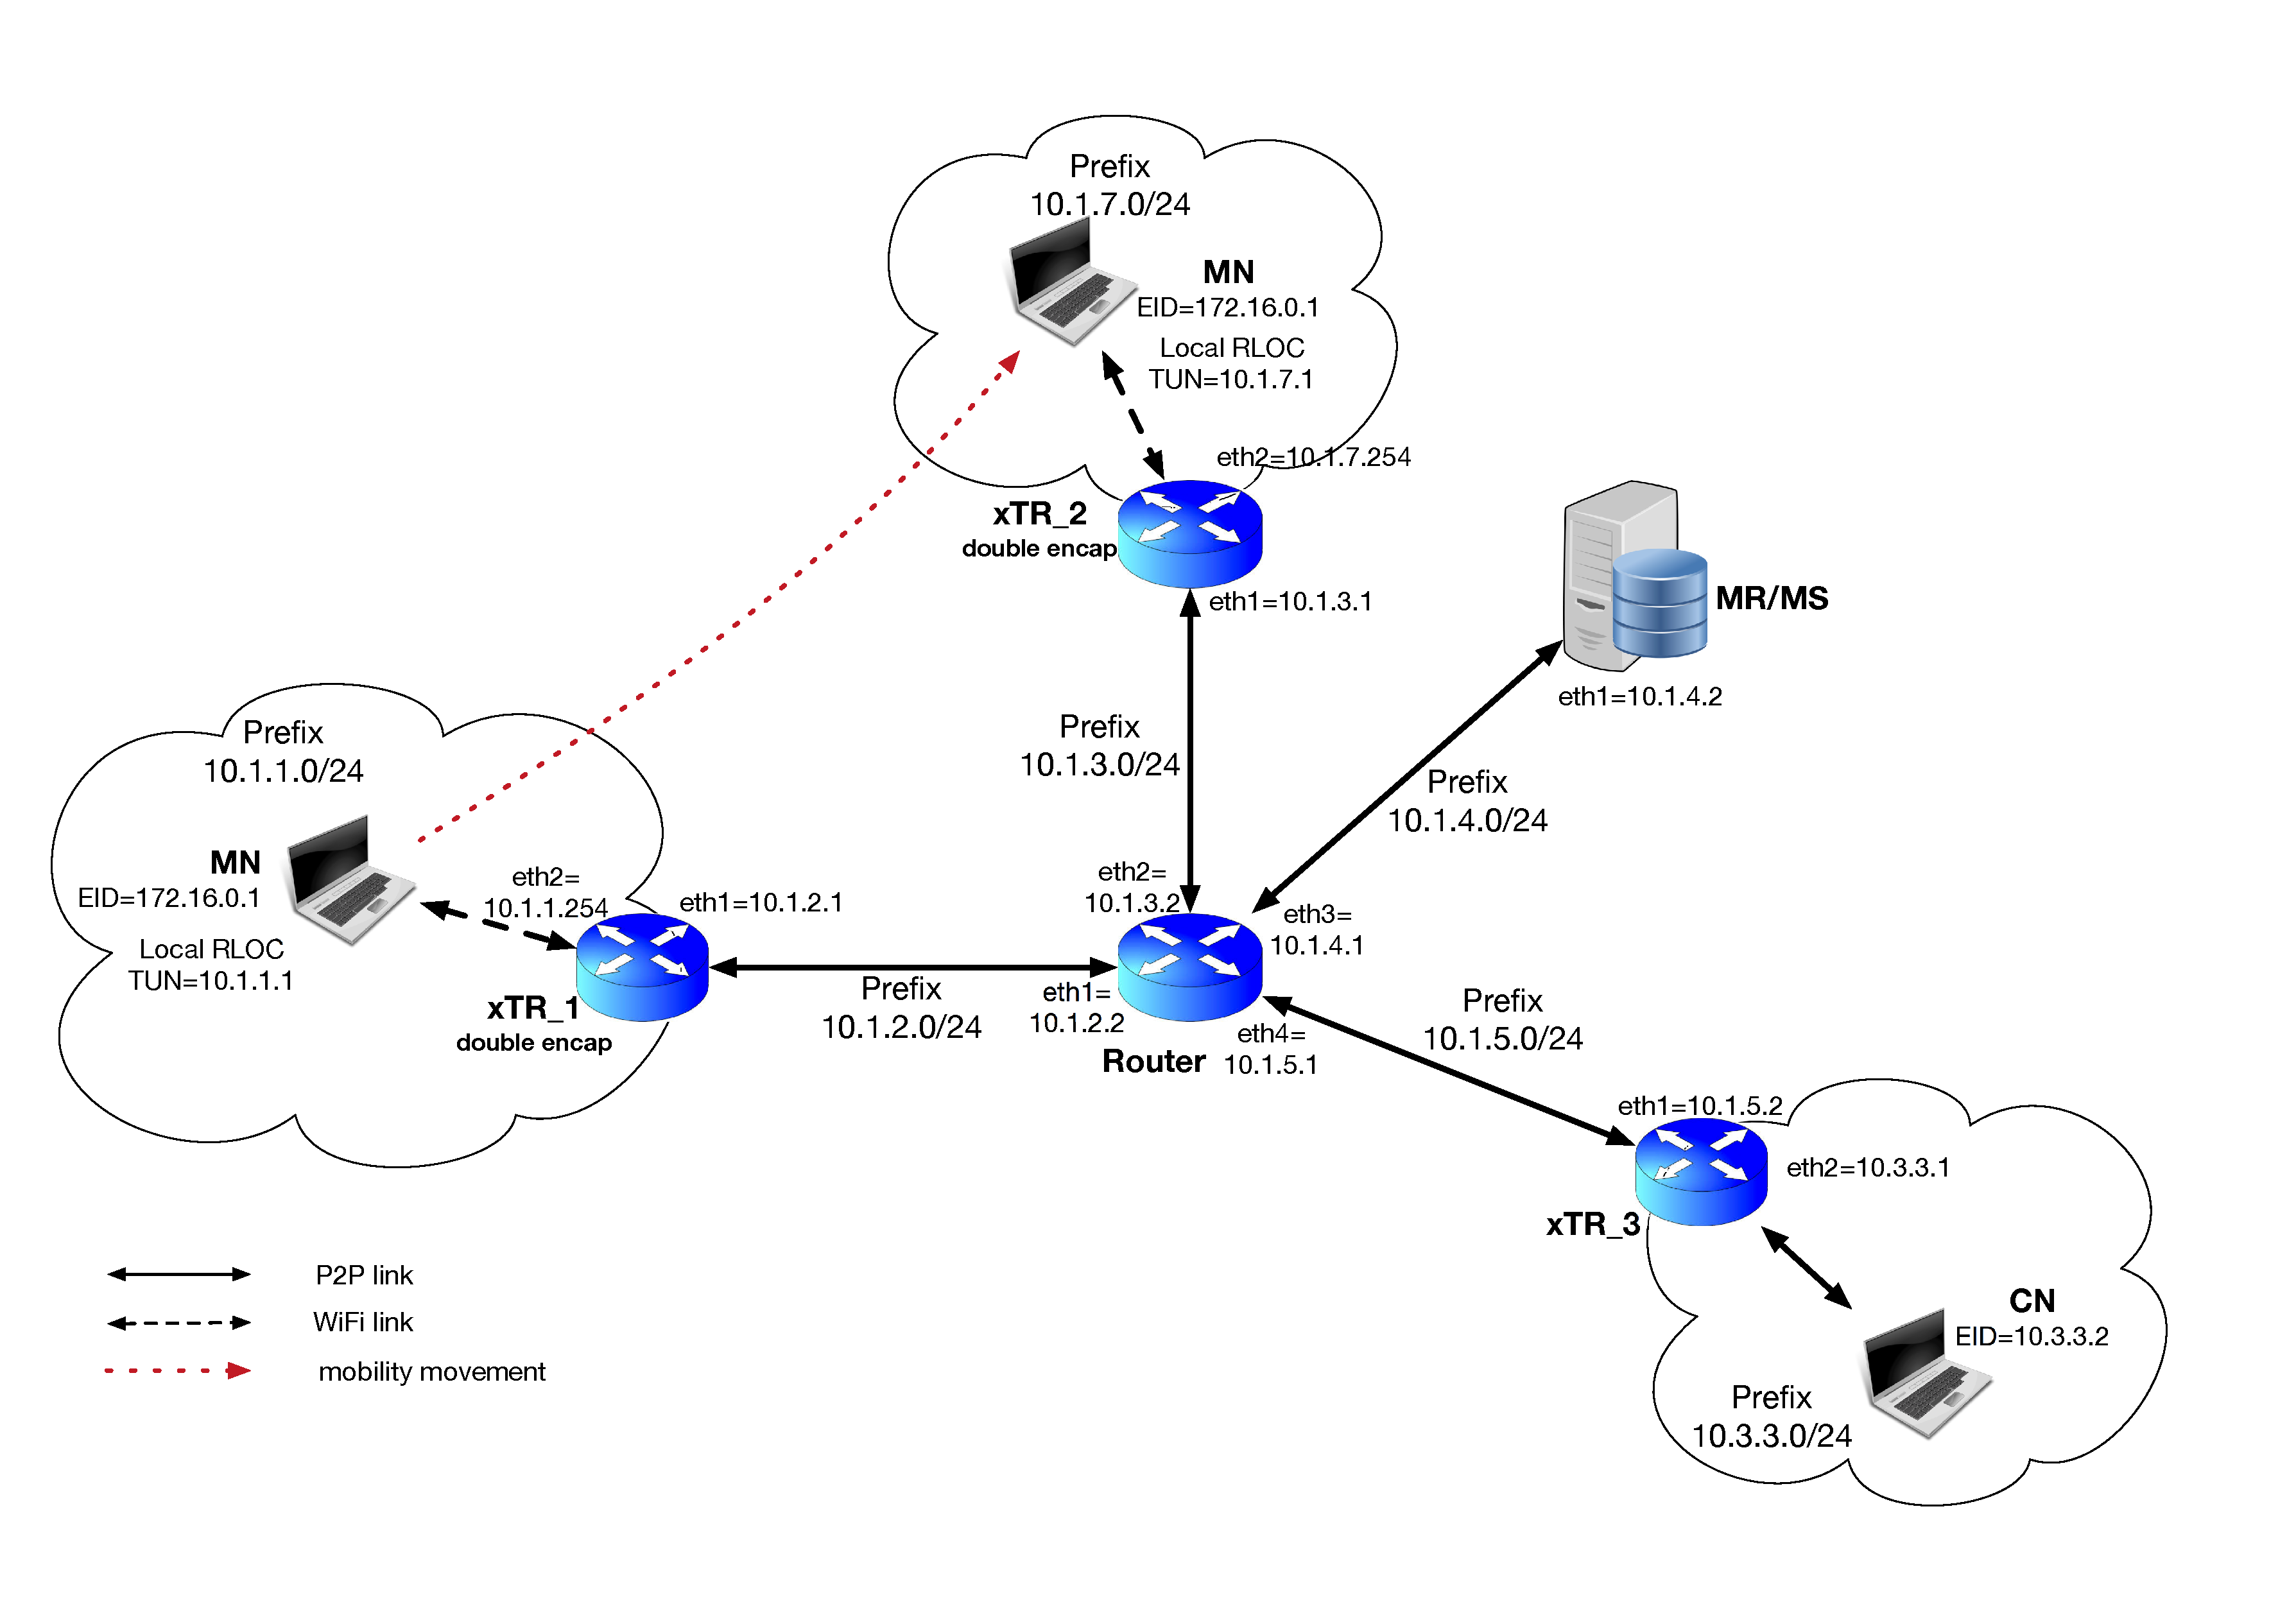
\includegraphics[width=\textwidth]{Pics/mobility_through_subnets_2_encap_topo}
	\caption{LISP mobility simulation scenario for double encapsulation}
	\label{sim_scenario}
\end{figure}
%-< END FIGURE >--------------------------------------------------------------------

%-< SUB SECTION >--------------------------------------------------------------------
\subsection{Simulation Setup}
\label{subsec:ns3_setup_lispmn_xTR}
%\begin{itemize}
%    \item Topology of simulation setup
%    \item The simulation parameter settings
%\end{itemize}
In our simulation, a LISP-MN with permanent EID 172.16.0.1 is initially placed in network 10.1.1.0/24. An \emph{echo} application on LISP-MN sends one packet per second to a remote stationary node CN with EID 10.3.3.2, and the LISP-MN moves into network 10.1.7.0/24 at speed of $7.07m/s$. The distance between xTR\_1 and xTR\_2 is $170m$. LISP-MN node uses Wi-Fi to connect to xTR\_1. At a certain moment during the moving, the Wi-Fi link between LISP-MN and xTR\_1 is down, which triggers the handover procedure. Afterwards, LISP-MN connects to xTR\_2 and reestablishes the communication with CN node. The total simulation time is set to $45s$ and the DHCP procedure delay is set to $1s$. We conduct many times of simulations with the various beacon interval of Wi-Fi channel in the range of $0.05s$ to $2s$.

%-< SUB SECTION >--------------------------------------------------------------------
\subsection{Results}
\label{sec:ns3_results_lispmn_xTR}
%\begin{itemize}
%    \item Show that LISP-MN procedure passes successfully
%    \item Show that the handover delay in LISP-MN handover procedure
%\end{itemize}
As shown in Fig.~\ref{sim_schema_LISPMN_xTR}, when MN sending the packets to CN during the simulation, it needs double encapsulation and the packet flow sequences are as follows. The traditional IP packets with EID 172.16.0.1 as source address and EID 10.3.3.2 as destination address are encapsulated by adding Local RLOC 10.1.1.1 as outer source address and RLOC 10.1.5.2 as outer destination address after MN querying the mapping information to MR. The LISP packets are encapsulated and forwarded to xTR\_1. The latter gets the mapping information from MR and encapsulates the packets again by adding the RLOC 10.1.2.1 as the outer source address and RLOC 10.1.5.2 as the outer destination address, then sends the packets on Internet core. The xTR\_3 needs dencapsulate the packets twice after it receiving and verifying the packets, and finally sends to CN. Once LISP-MN lost its Wi-Fi connection with xTR\_1, it needs a DHCP procedure (consisting of DHCP Discover, DHCP Offer, DHCP Request and DHCP ACK) with xTR\_2 to get a new LRLOC 10.1.7.1 and then triggers LISP SMR to xTR\_3. After xTR\_3 getting new mapping information of <10.1.7.1, 10.1.3.1> and <172.16.0.1, 10.1.7.1>, the connection between LISP-MN and CN is re-established again.
%-< FIGURE >--------------------------------------------------------------------
\begin{figure}[!th]
	\centering
	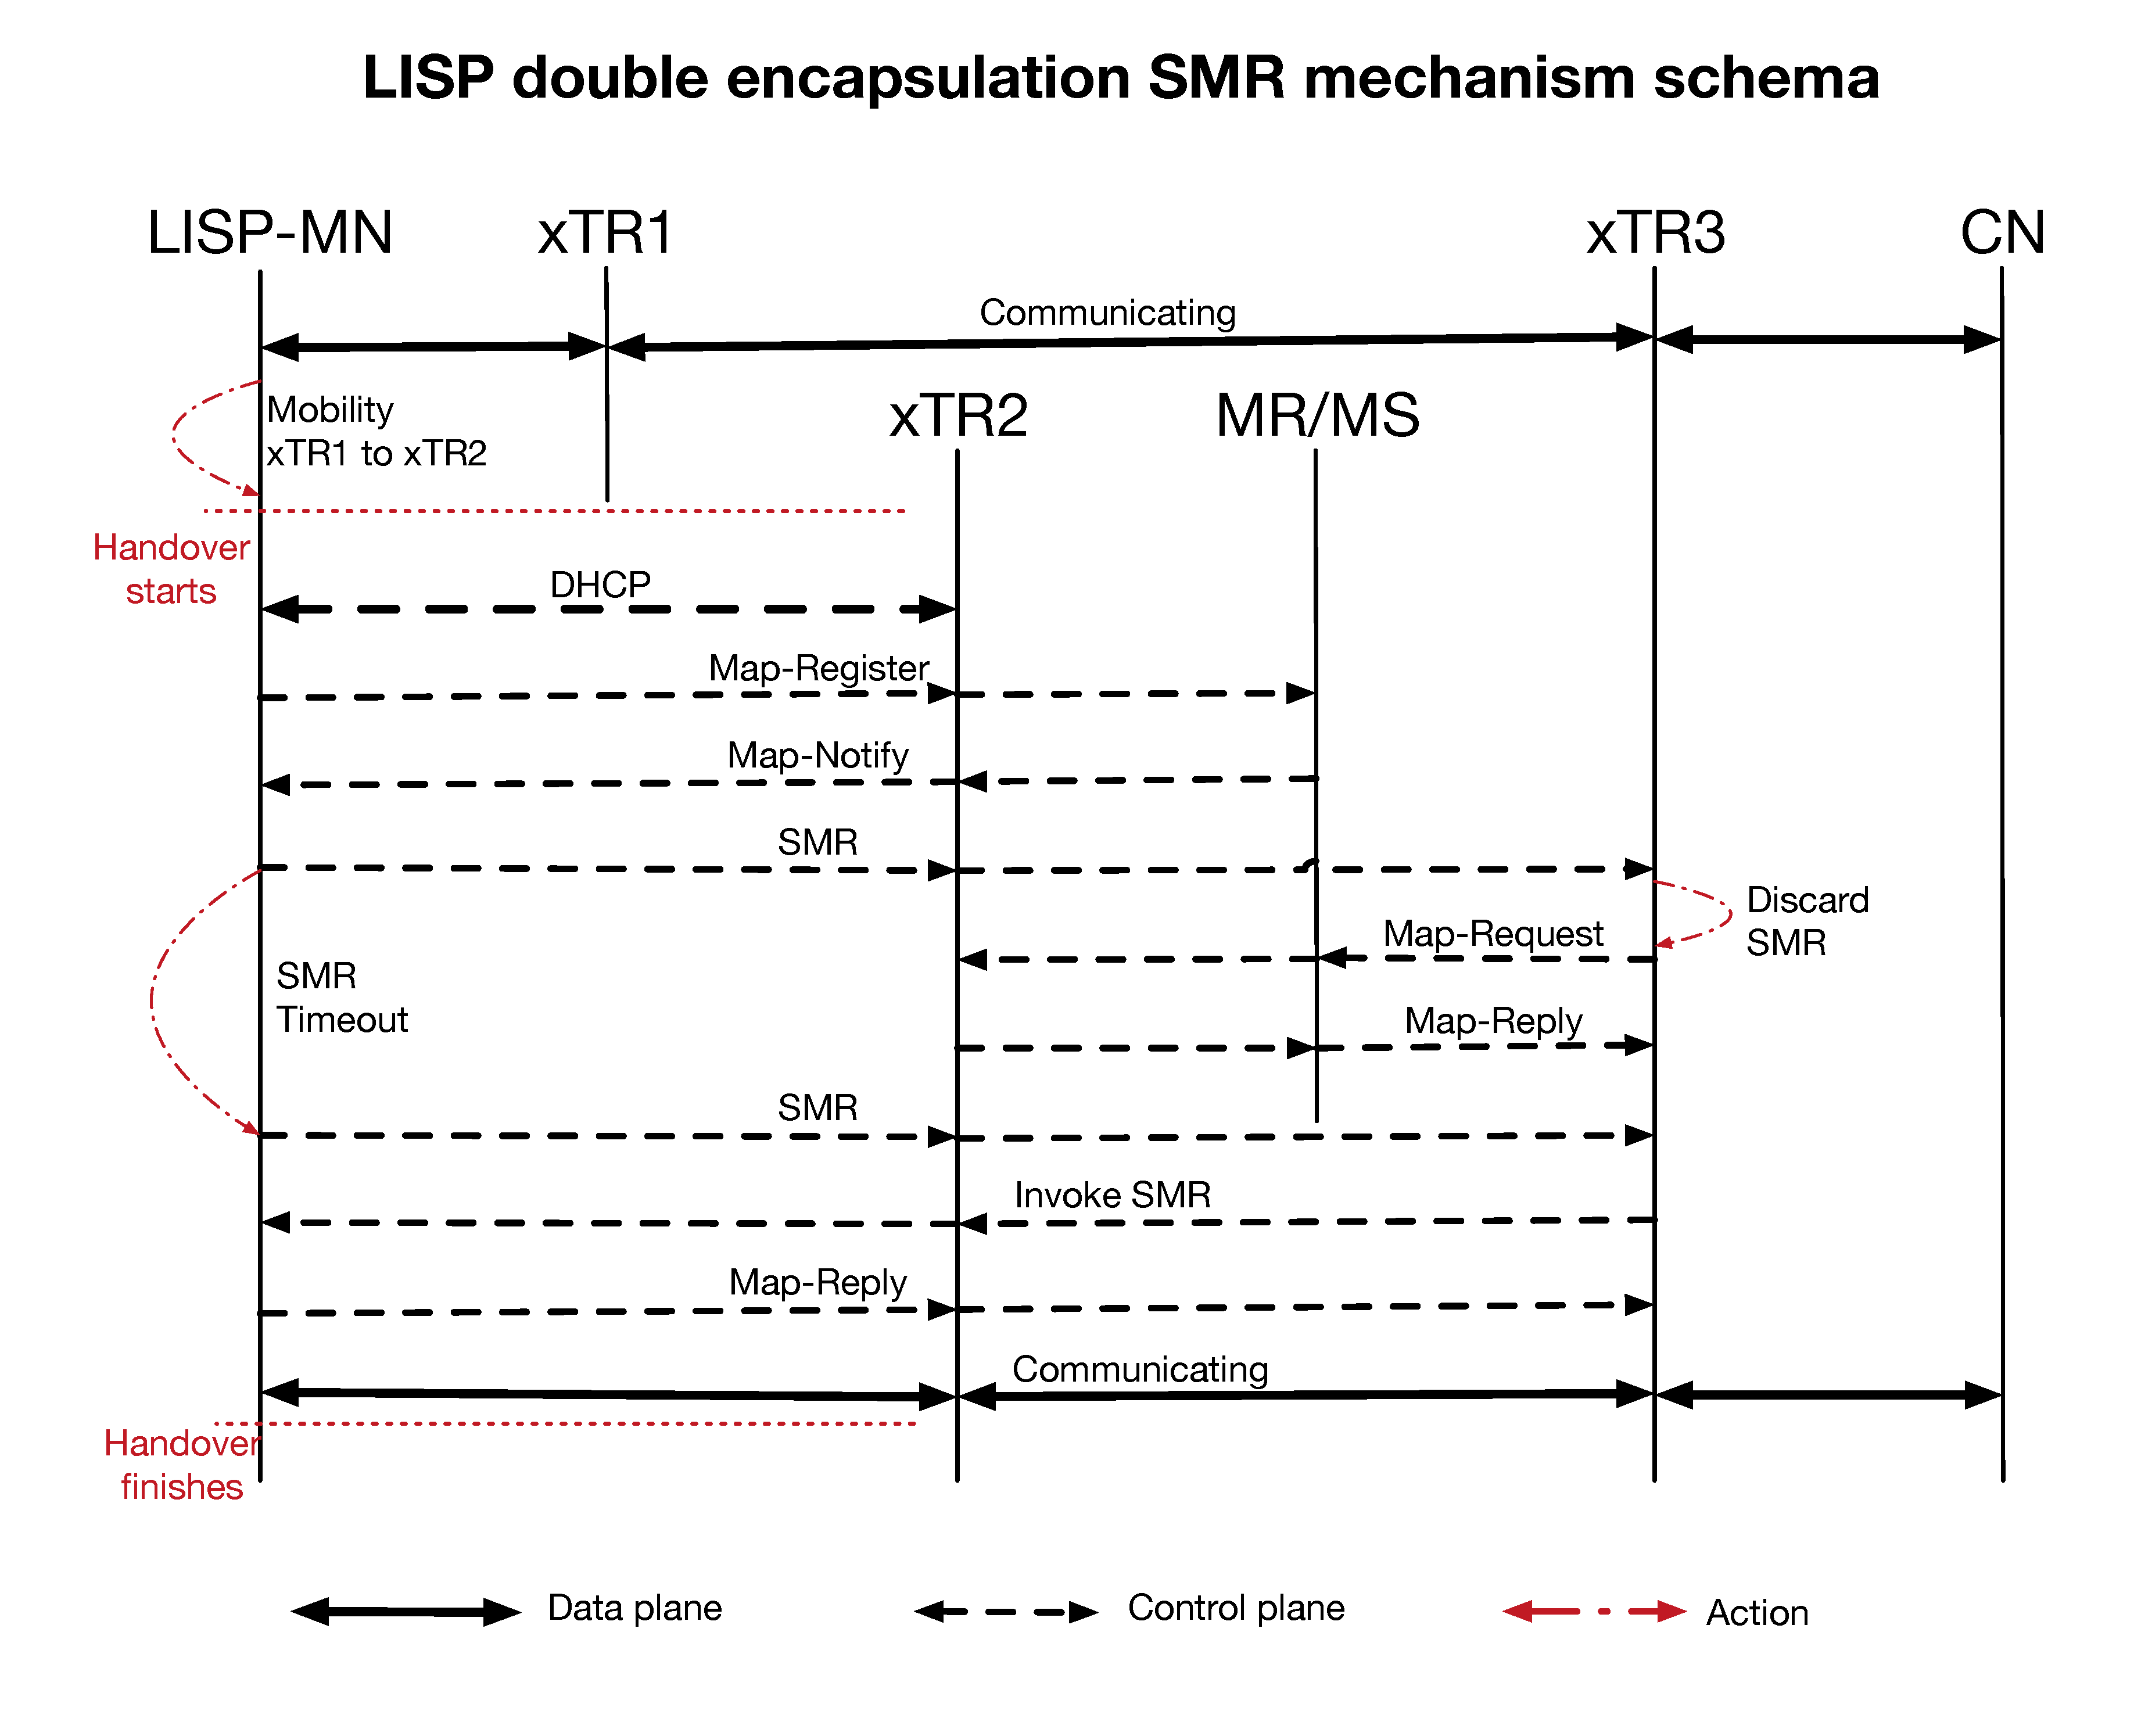
\includegraphics[width=\textwidth]{Pics/Mobility_LISPMN_xTR_schema_SMR_simplify}
	\caption{Schema for LISP-MN in LISP-Site mobility}
	\label{sim_schema_LISPMN_xTR}
\end{figure}
%-< END FIGURE >--------------------------------------------------------------------

%-< FIGURE >--------------------------------------------------------------------
\begin{figure}[!th]
	\centering
	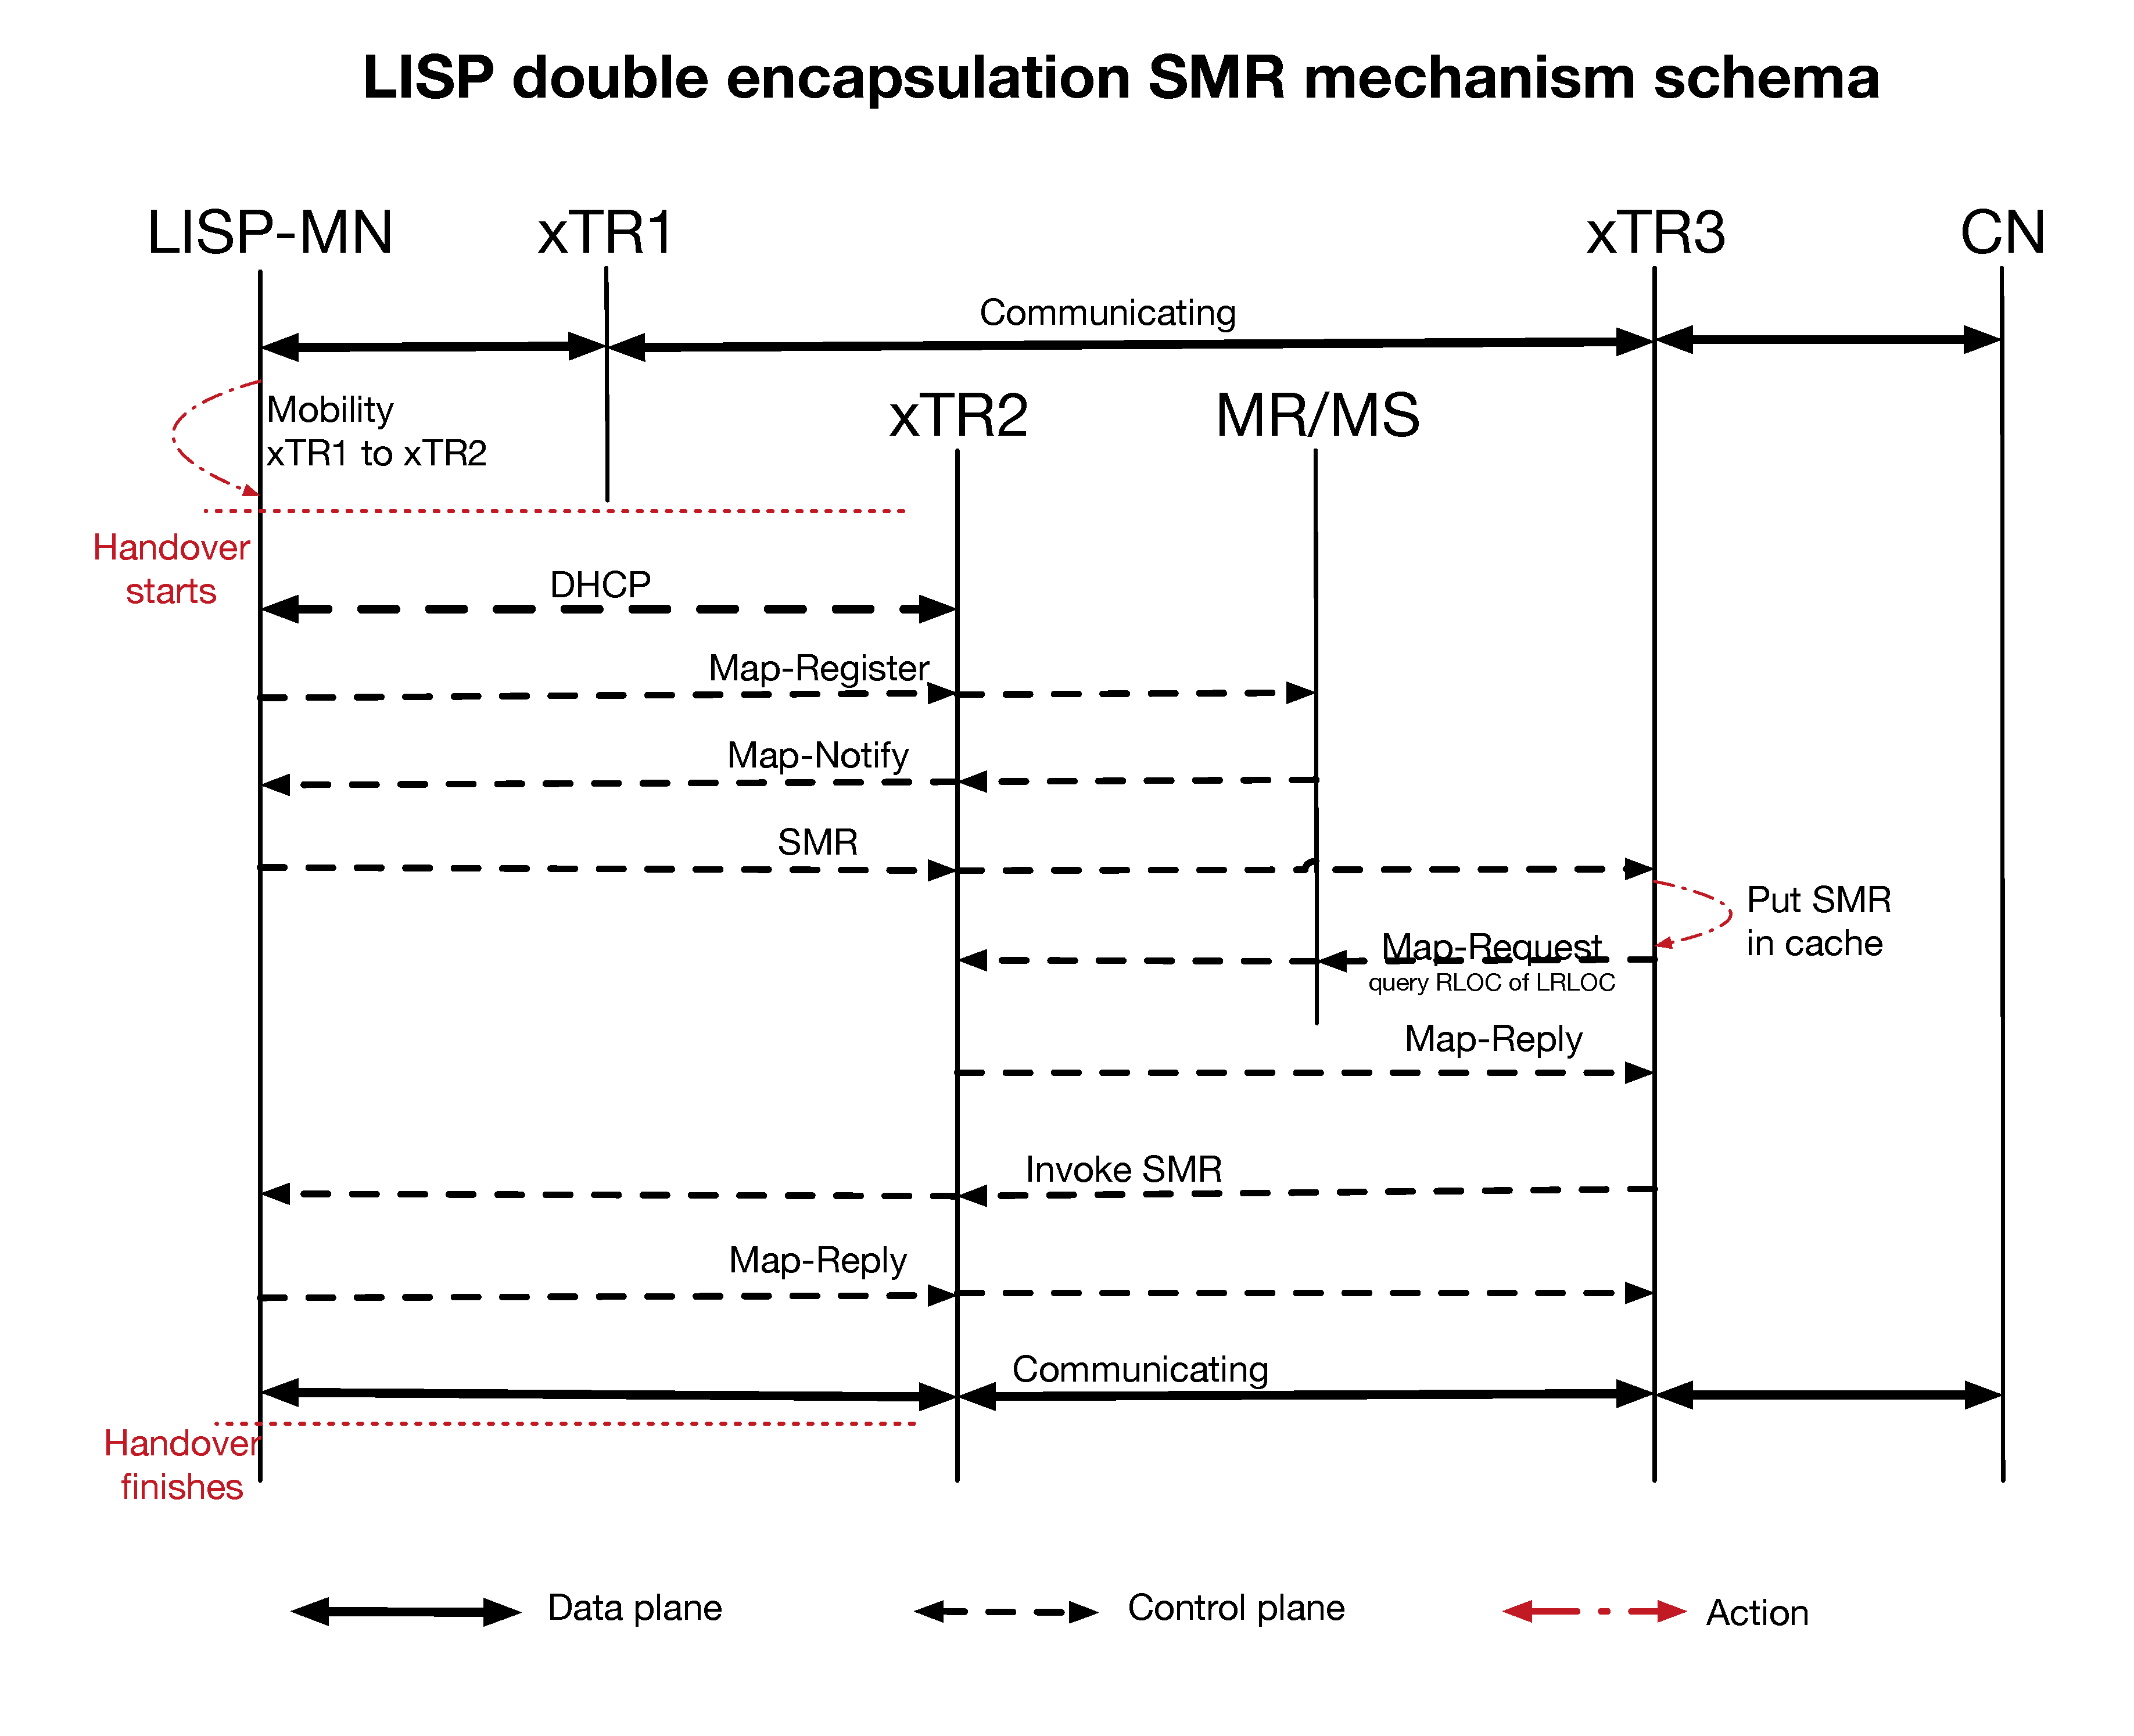
\includegraphics[width=\textwidth]{Pics/Mobility_LISPMN_xTR_schema_SMR_improving_simplify}
	\caption{Schema for improving LISP-MN in LISP-Site mobility}
	\label{sim_schema_LISPMN_xTR_improving}
\end{figure}
%-< END FIGURE >--------------------------------------------------------------------
Fig.~\ref{sim_schema_LISPMN_xTR_improving}

%-< TABLE >-----------------------------------------------------------------
\begin{table}[!tb]
	\centering
	\caption{Different configurations of probes in 2015}
	\label{Probes_config_2015}{
		% \resizebox{0.9\textwidth}{!}{%
		\begin{tabular}{@{}|c|c|@{}}
			\hline\hline
			Parameters & Descriptions   \\ \hline
			$D_{overall}$ & Overall handover delay	\\  \hline    
			$D_{DHCP}$ &  DHCP address configuration delay \\  \hline    
			$D_{Register}$ &  Delay of sending Map-Register      	\\  \hline
			$D_{Notify}$ &  Delay of receiving Map-Notify      	\\  \hline           
			$D_{Request}$ &  Delay of sending Map-Request to MDS      	\\  \hline   
			$D_{Reply}$ &  Delay of receiving Map-Reply      	\\  \hline      
			$D_{Resolve}$ &  Delay of resolving mapping information in MDS      	\\  \hline               
			$D_{SMR}$ &  Delay of sending SMR       	\\  \hline 
			$D_{invokeSMR}$ &  Delay of sending invoke-SMR \\  \hline 
			$D_{CheckAlive}$ &  Delay of checking connection of MN      	\\  \hline
			$T_{A-B}$ &  Delay of packet transmission between A and B     	\\  \hline
			$T_{timeout_SMR}$ &  Timeout of SMR     	\\  \hline
			$T_{timeout_ping}$ &  Timeout of ping     	\\  \hline  \hline               
		
	\end{tabular}
	}
\end{table}
%-< END TABLE >-----------------------------------------------------------------

The overall handover delay in this paper is defined at the moment that LISP-MN sending DHCP Discover message to xTR\_2 and end up with xTR\_3 receiving the last Map-Reply from xTR\_2. Precisely, it is composed by three parts: the Wi-Fi association delay, the DHCP related delay and LISP SMR delay:
\begin{eqnarray}
D_{overall} &=& D_{DHCP} + D_{Register} + D_{Notify} + D_{SMR} + T_{timeout_SMR} + D_{SMR} + D_{invokeSMR} + D_{Reply} \nonumber \\
&=& D_{DHCP} + 2T_{LISPMN-MDS} + 4T_{LISPMN-xTR_3} + T_{timeout_SMR}\nonumber \\
&=& D_{DHCP} + 2* (3*2ms) + 4*(3*2ms) + 3s\nonumber \\
&=& D_{DHCP} + 3036 ms
\end{eqnarray}
During $T_{timeout\_SMR}$ (normally is 3 seconds), xTR\_3 queries the mapping system for the RLOC of LISP-MN LRLOC.


\begin{eqnarray}
	D_{overall} &=& D_{DHCP} + D_{Register} + D_{Notify} + D_{SMR} + D_{Request} + D_{Reply} + D_{invokeSMR} + D_{Reply} \nonumber \\
	&=& D_{DHCP} + 2T_{LISPMN-MDS} + T_{xTR_3-MDS} + D_{Resolve} + 3T_{LISPMN-xTR_3} + T_{xTR_2-xTR_3} \nonumber \\
	&=& D_{DHCP} + 2* (3*2ms) + 2*2ms + 200ms + 3*(3*2ms) + 2*2ms \nonumber \\
	&=& D_{DHCP} + 238 ms
\end{eqnarray}
where $D$ is the delay, $BI$ is Beacon Interval, subscriptions $Wi-Fi$, $DHCP$ and $SMR$ respectively refers to Wi-Fi association, DHCP procedure and LISP SMR. (Min value of handover delay = 1.300349, where packet sending interval = 0.02 s) 

After several executions of simulation program, we observe that the overall handover delay changes by the various beacon intervals, in particular the Wi-Fi association delay depends on the different beacon intervals, whereas LISP SMR procedure always cost around $3s$. To get the lower bound of overall handover delay, we can ignore the Wi-Fi association delay when the beacon interval is $500ms$, and the latency due to DHCP procedure is always $1s$. Thus, adopting LISP-MN to conduct the host-based mobility takes at least $4s$. Compared to current most stable solution for host-based IP mobility management MIPv6, which latency including L2 and L3 in a real Wi-Fi testbed is around $3.68s$~\cite{vassiliou2010analysis}, LISP-MN has a higher delay caused by the double encapsulation mechanism introduced by LISP-MN behind LISP-Site. 

During handover, CN can successfully receive packets from LISP-MN right after DHCP procedure being accomplished, but LISP-MN cannot receive the packets from CN until LISP SMR procedure is also finished. Thus, during DHCP procedure, all bi-directional transmitted packets are lost. To improve the performance, \cite{tang2017lisp} proposes a network-level LISP-MN solution, but has not validated their proposals neither in simulation nor in testbed. Our ns-3 implementation can be used to realize them.

%-< FIGURE >--------------------------------------------------------------------
\begin{figure}[!th]
	\centering
	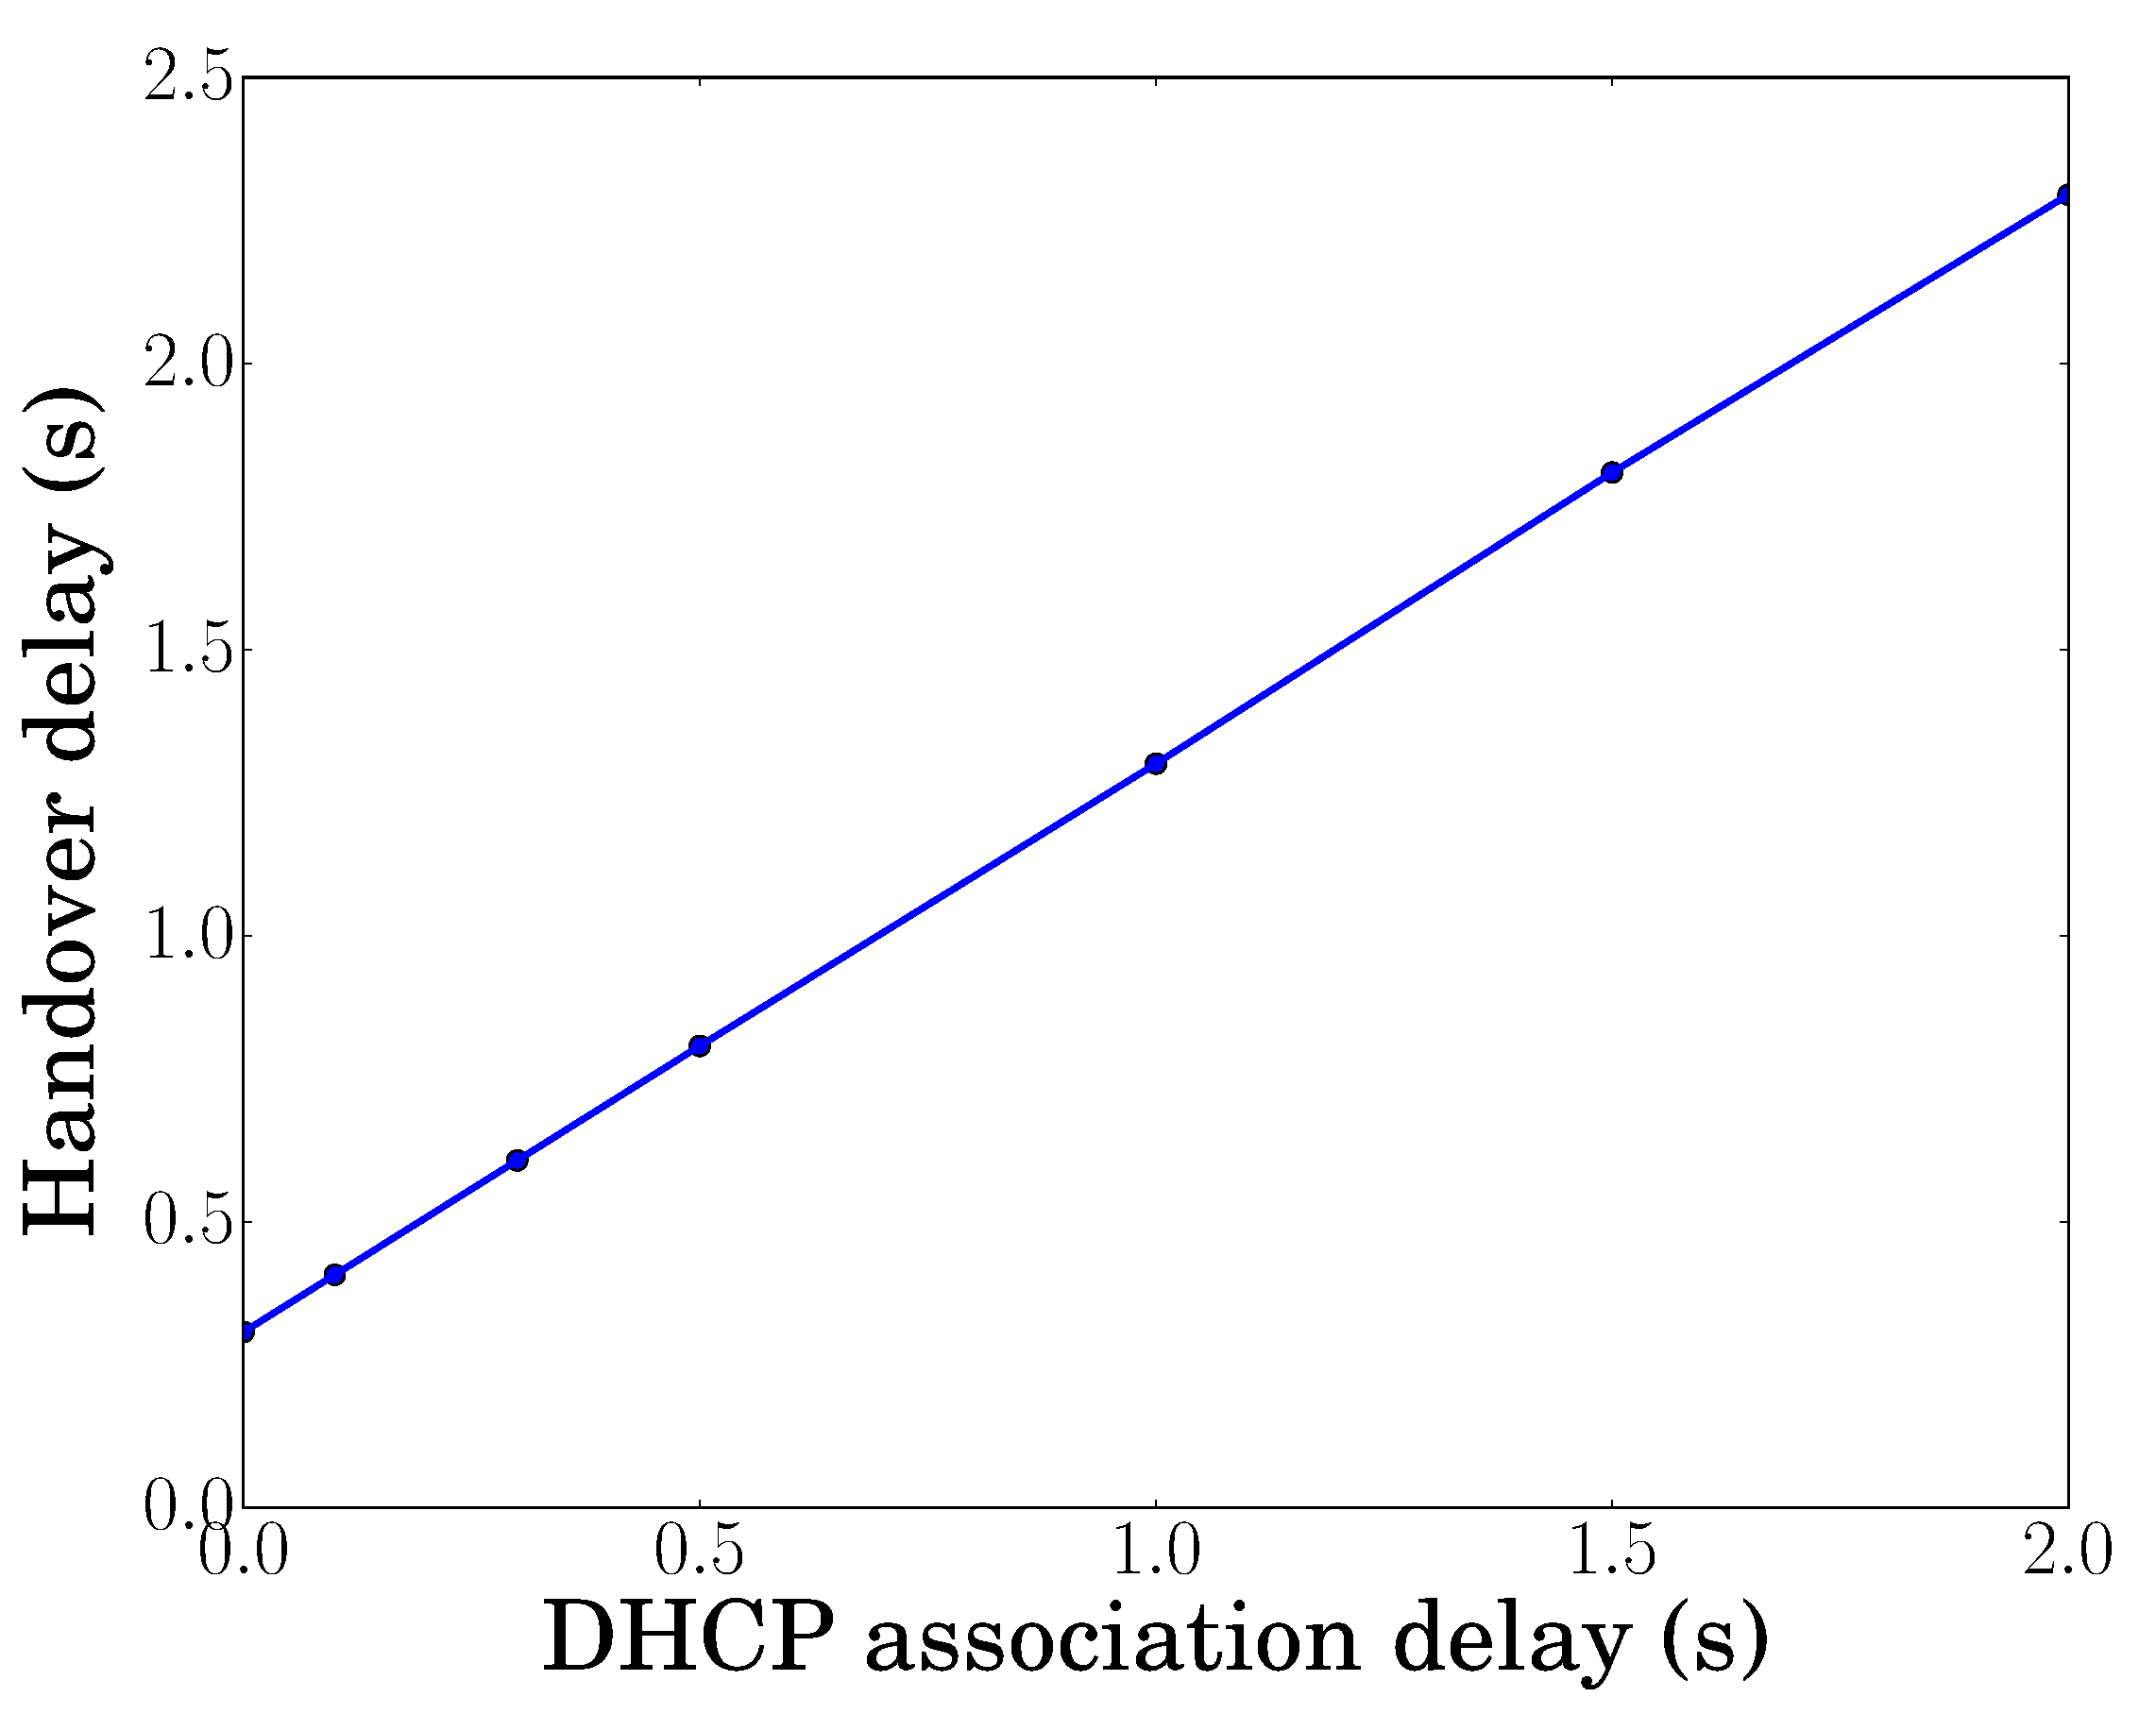
\includegraphics[width=0.7\textwidth]{Pics/LISP_mobility_double_encap_DHCP}
	\caption{Impact of DHCP association on handover delay}
	\label{LISP_mobility_double_encap_DHCP}
\end{figure}
%-< END FIGURE >--------------------------------------------------------------------


%-< FIGURE >--------------------------------------------------------------------
\begin{figure}[!th]
	\centering
	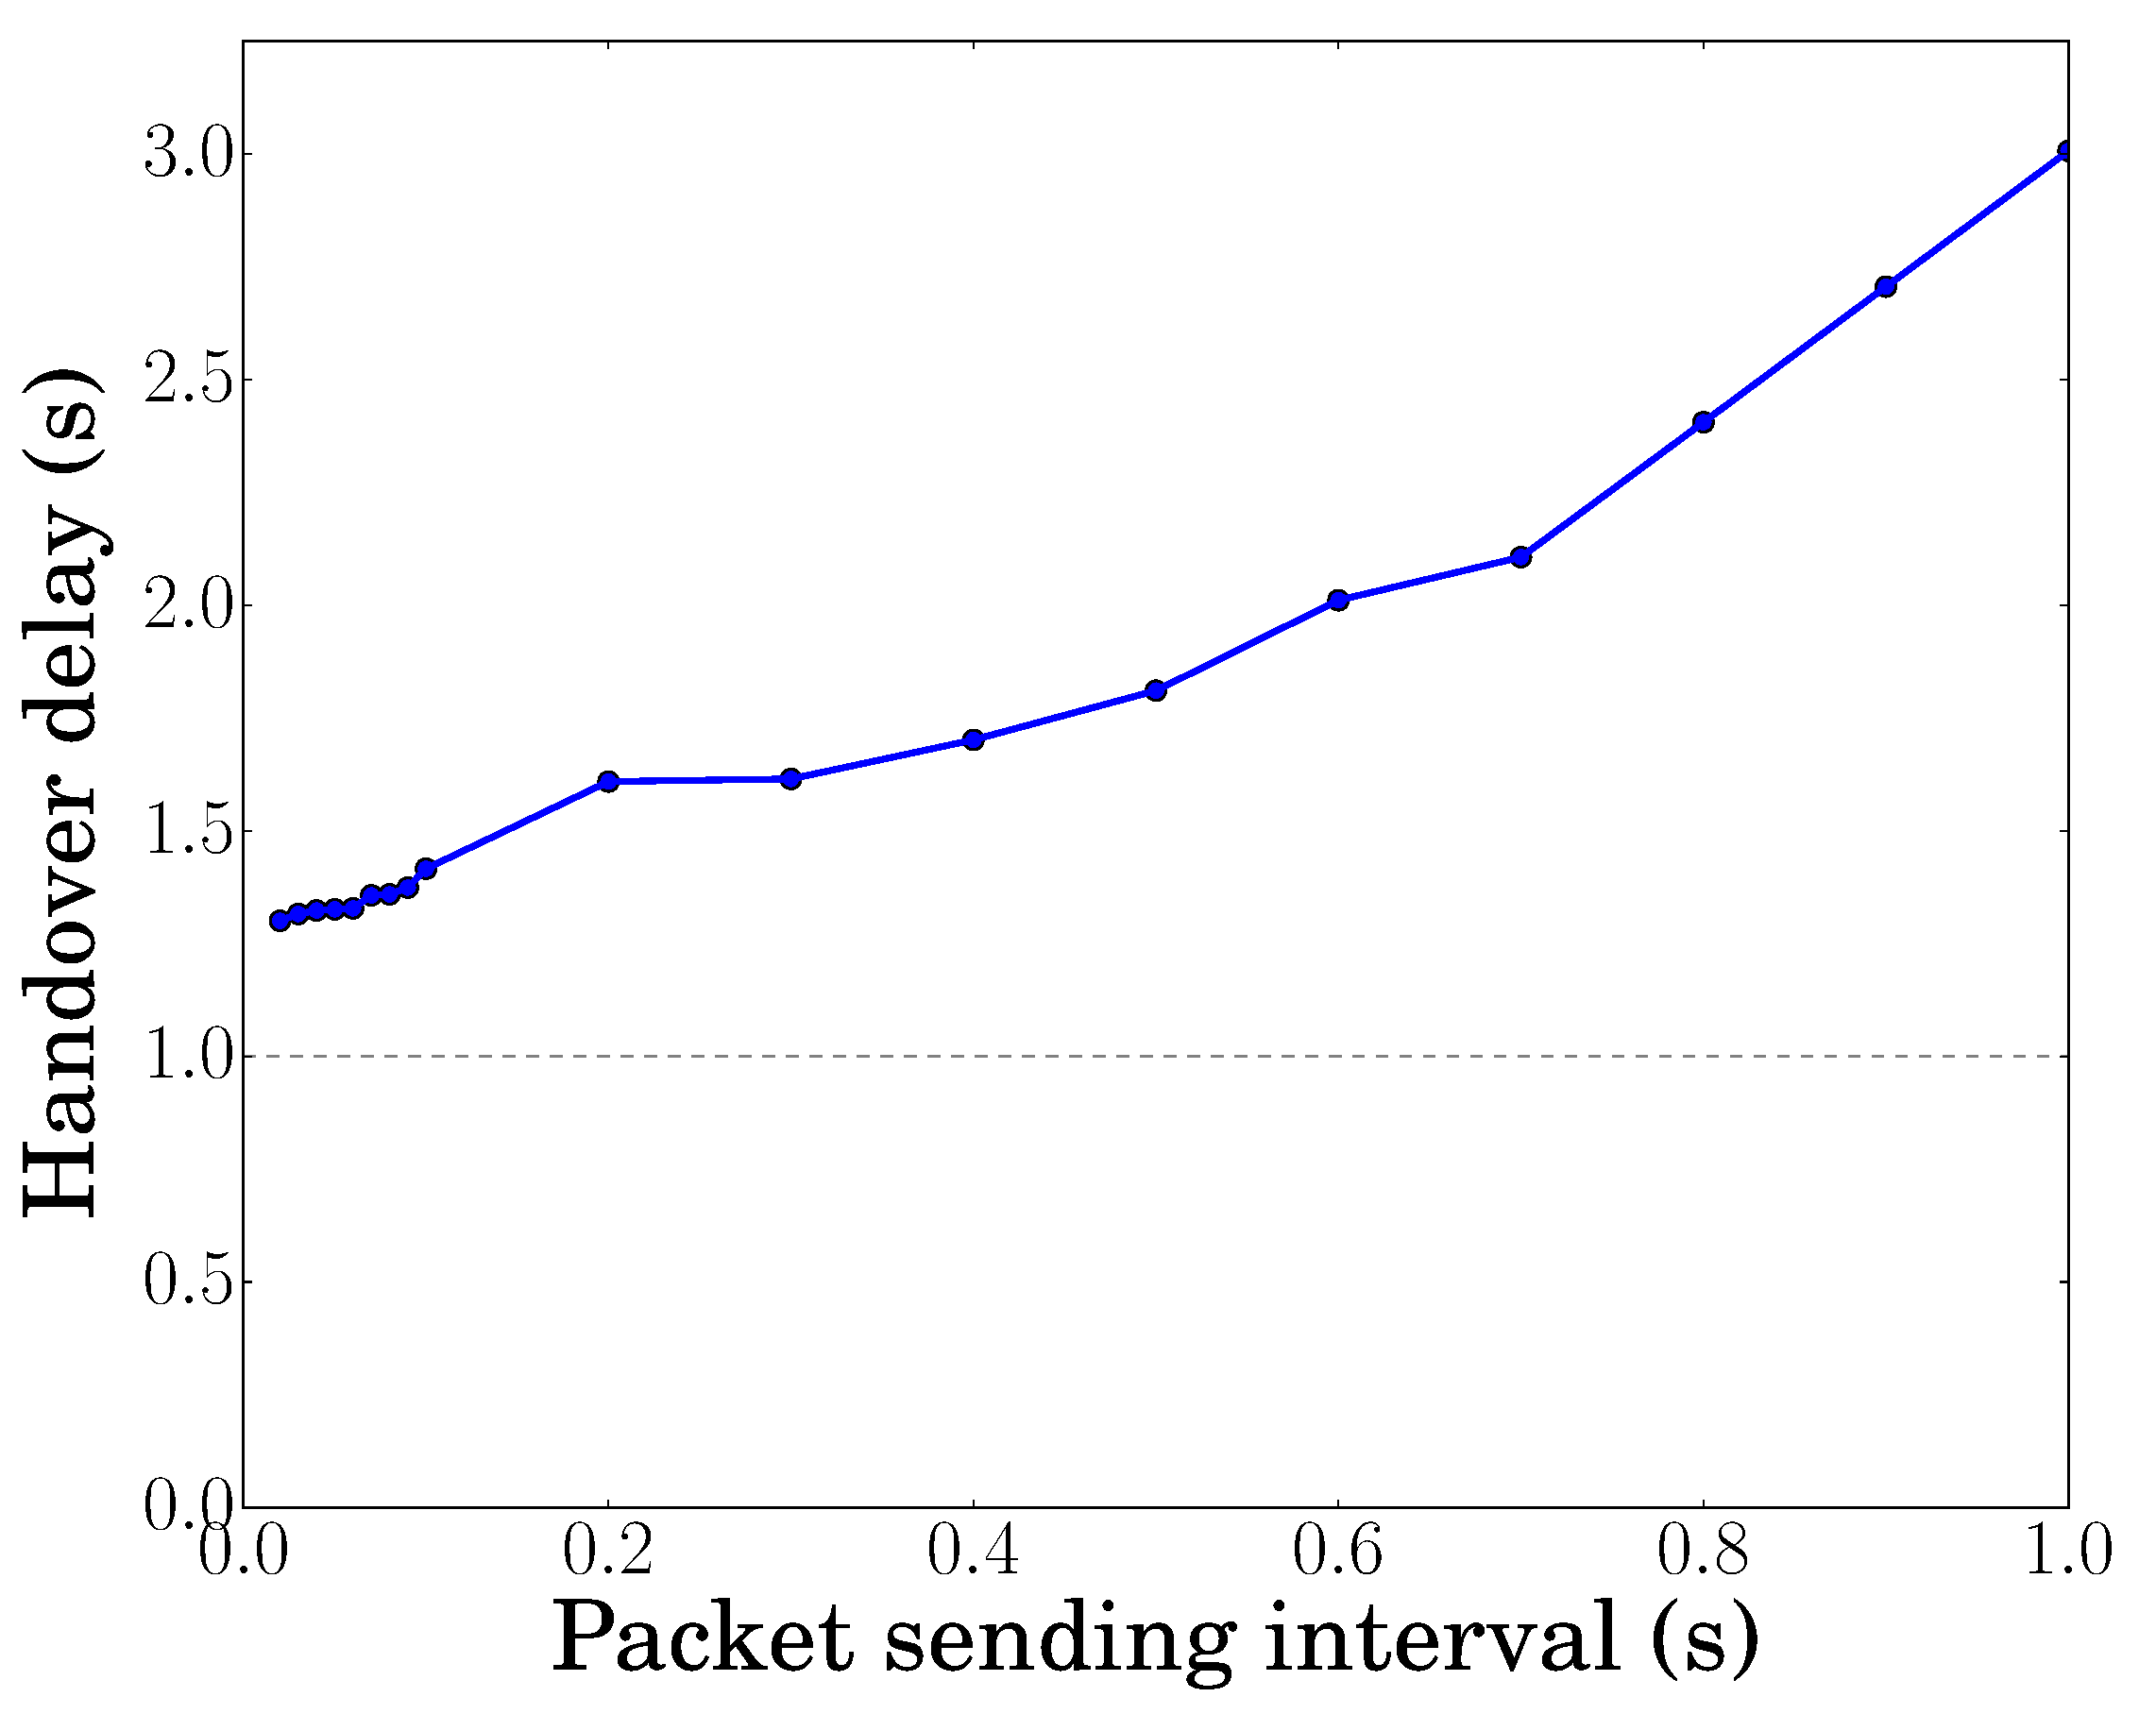
\includegraphics[width=0.7\textwidth]{Pics/LISP_mobility_double_encap_PacketInterval}
	\caption{Impact of packet sending interval on handover delay}
	\label{LISP_mobility_double_encap_PacketInterval}
\end{figure}
%-< END FIGURE >--------------------------------------------------------------------


%-< SECTION >--------------------------------------------------------------------
\section{Evaluation for LISP-MN in non-LISP-Site}
\label{sec:ns3_evaluation_lispmn}
We validate our LISP/LISP-MN implementation by conducting a simulation and providing a preliminary performance evaluation of handover delay. The simulation topology is shown in Fig.~\ref{sim_scenario}.
%-< FIGURE >--------------------------------------------------------------------
\begin{figure}[!th]
	\centering
	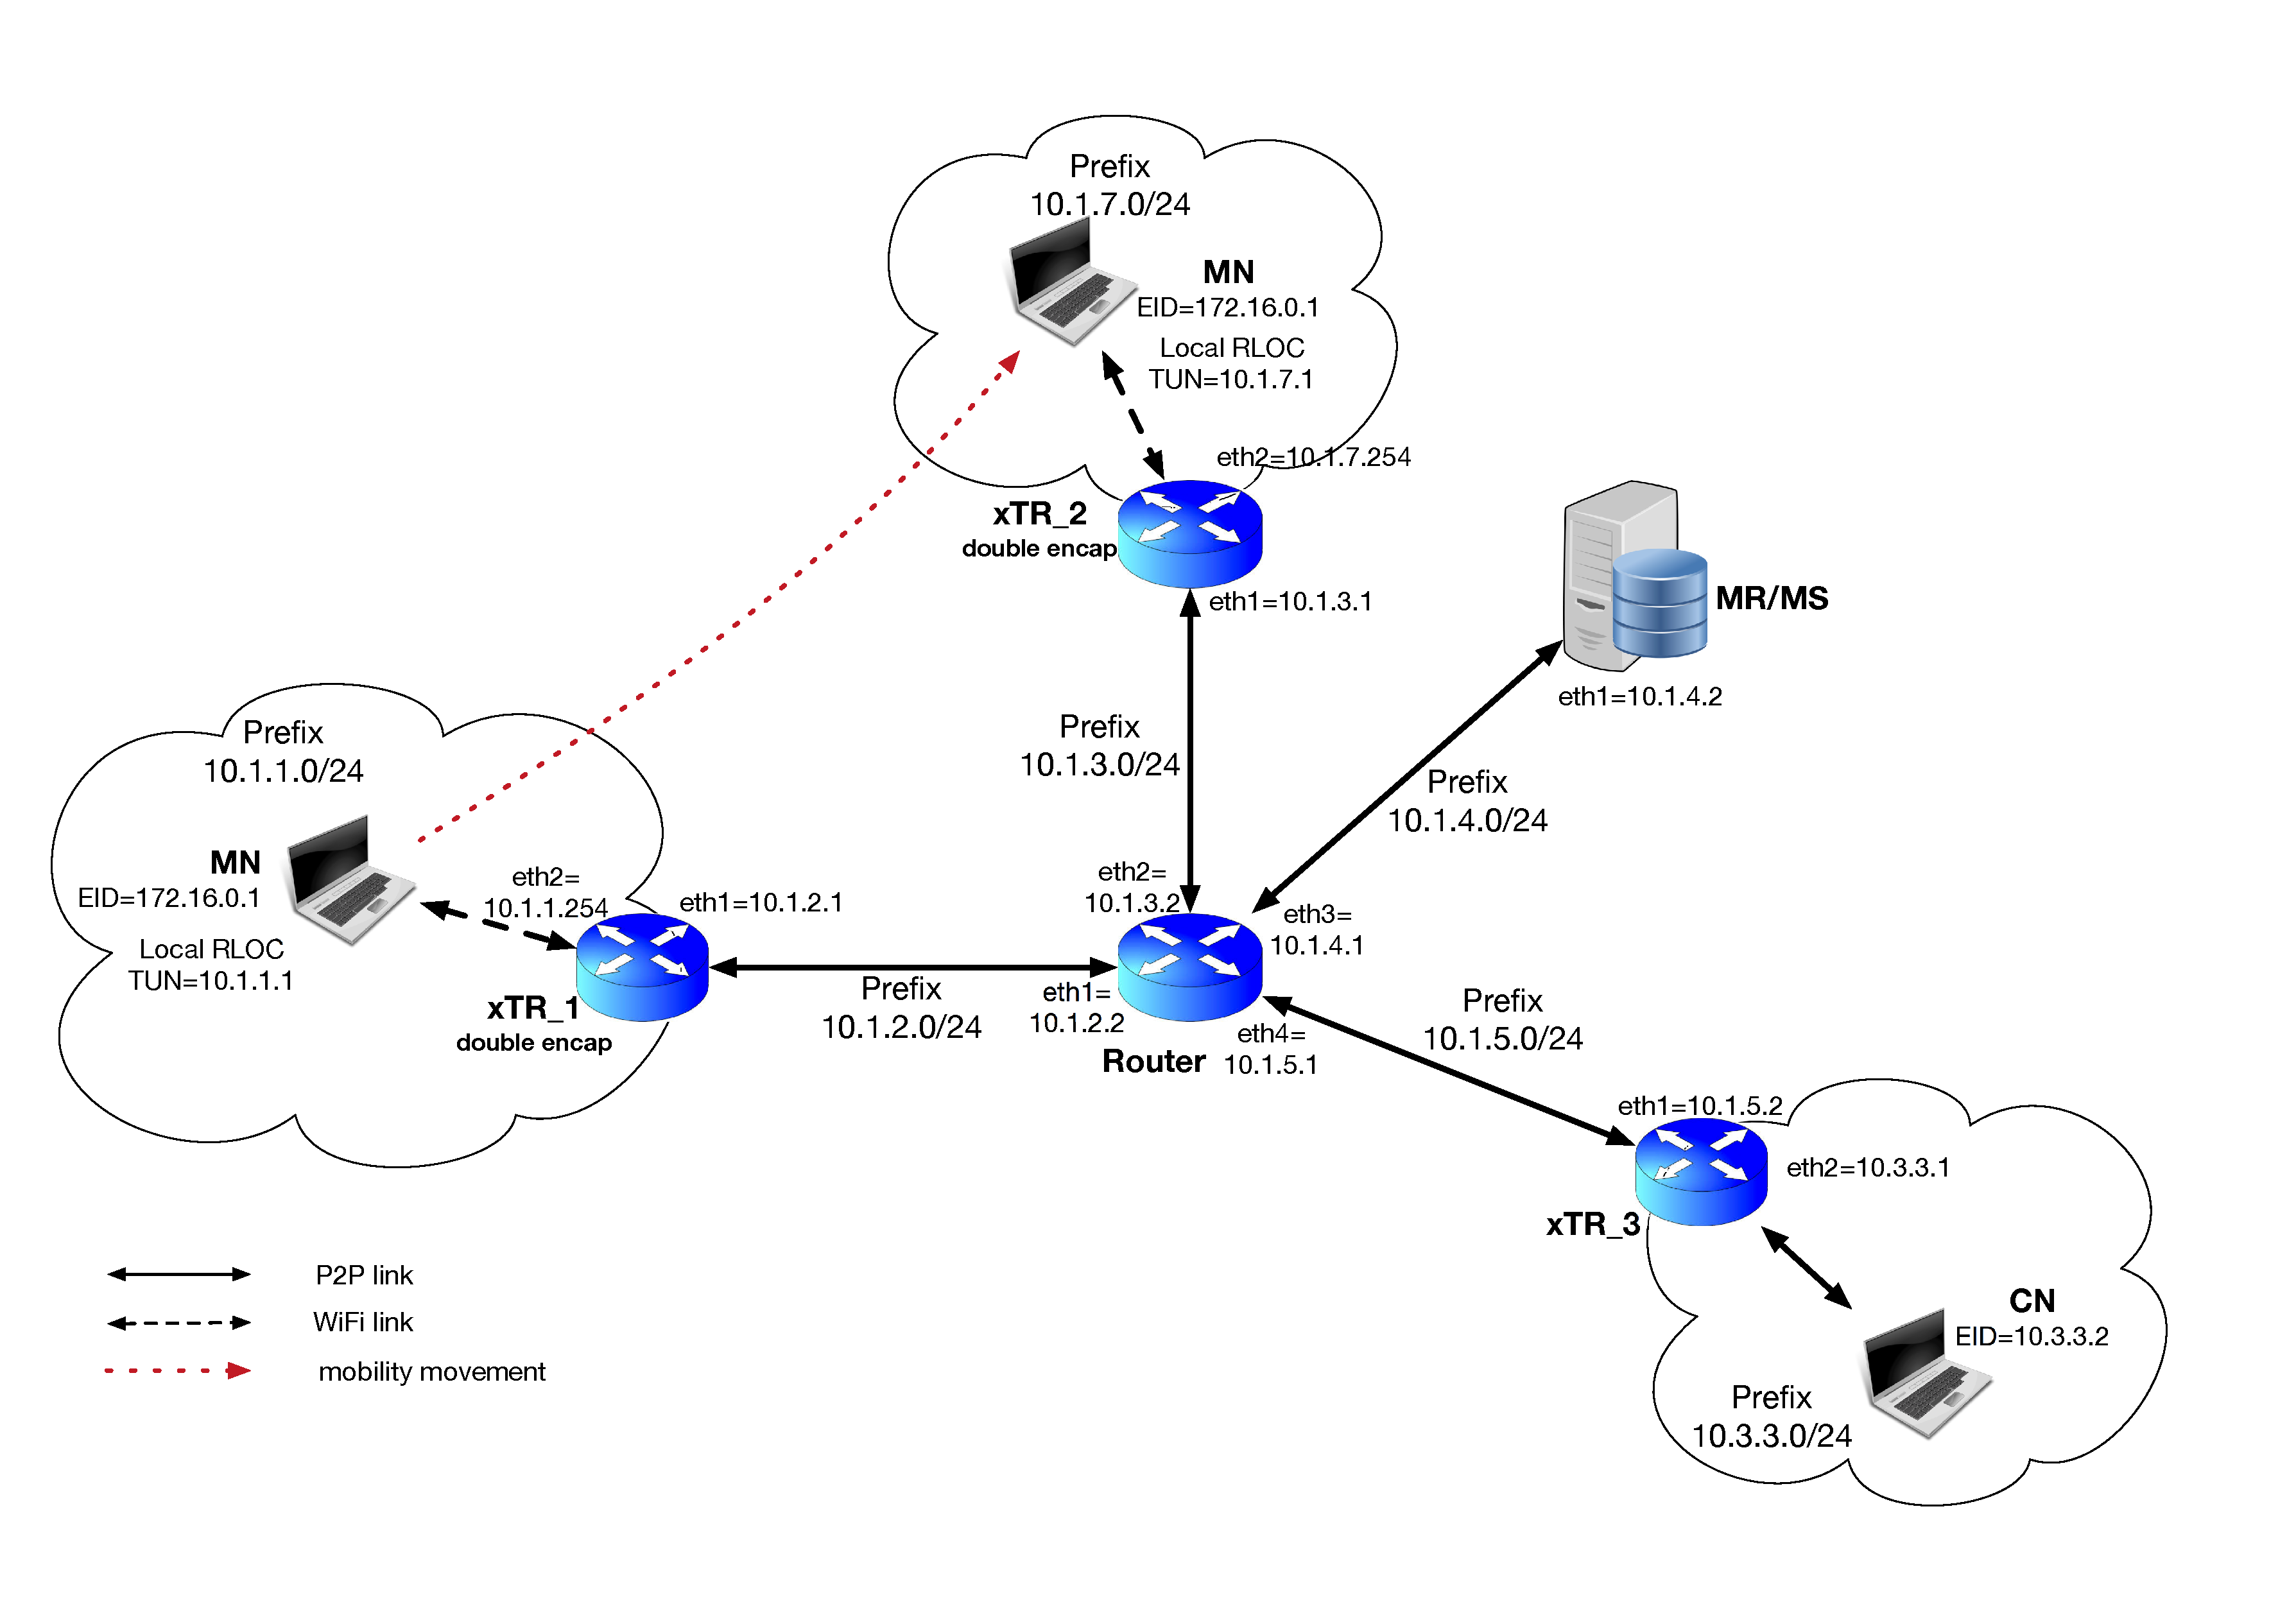
\includegraphics[width=\textwidth]{Pics/mobility_through_subnets_2_encap_topo}
	\caption{LISP mobility simulation scenario for double encapsulation}
	\label{sim_scenario}
\end{figure}
%-< END FIGURE >--------------------------------------------------------------------

%-< SUB SECTION >--------------------------------------------------------------------
\subsection{Simulation Setup}
\label{subsec:ns3_setup_lispmn}
%\begin{itemize}
%    \item Topology of simulation setup
%    \item The simulation parameter settings
%\end{itemize}
In our simulation, a LISP-MN with permanent EID 172.16.0.1 is initially placed in network 10.1.1.0/24. An \emph{echo} application on LISP-MN sends one packet per second to a remote stationary node CN with EID 10.3.3.2, and the LISP-MN moves into network 10.1.7.0/24 at speed of $7.07m/s$. The distance between xTR\_1 and xTR\_2 is $170m$. LISP-MN node uses Wi-Fi to connect to xTR\_1. At a certain moment during the moving, the Wi-Fi link between LISP-MN and xTR\_1 is down, which triggers the handover procedure. Afterwards, LISP-MN connects to xTR\_2 and reestablishes the communication with CN node. The total simulation time is set to $45s$ and the DHCP procedure delay is set to $1s$. We conduct many times of simulations with the various beacon interval of Wi-Fi channel in the range of $0.05s$ to $2s$.

%-< SUB SECTION >--------------------------------------------------------------------
\subsection{Results}
\label{sec:ns3_results_lispmn}

%-< FIGURE >--------------------------------------------------------------------
\begin{figure}[!th]
	\centering
	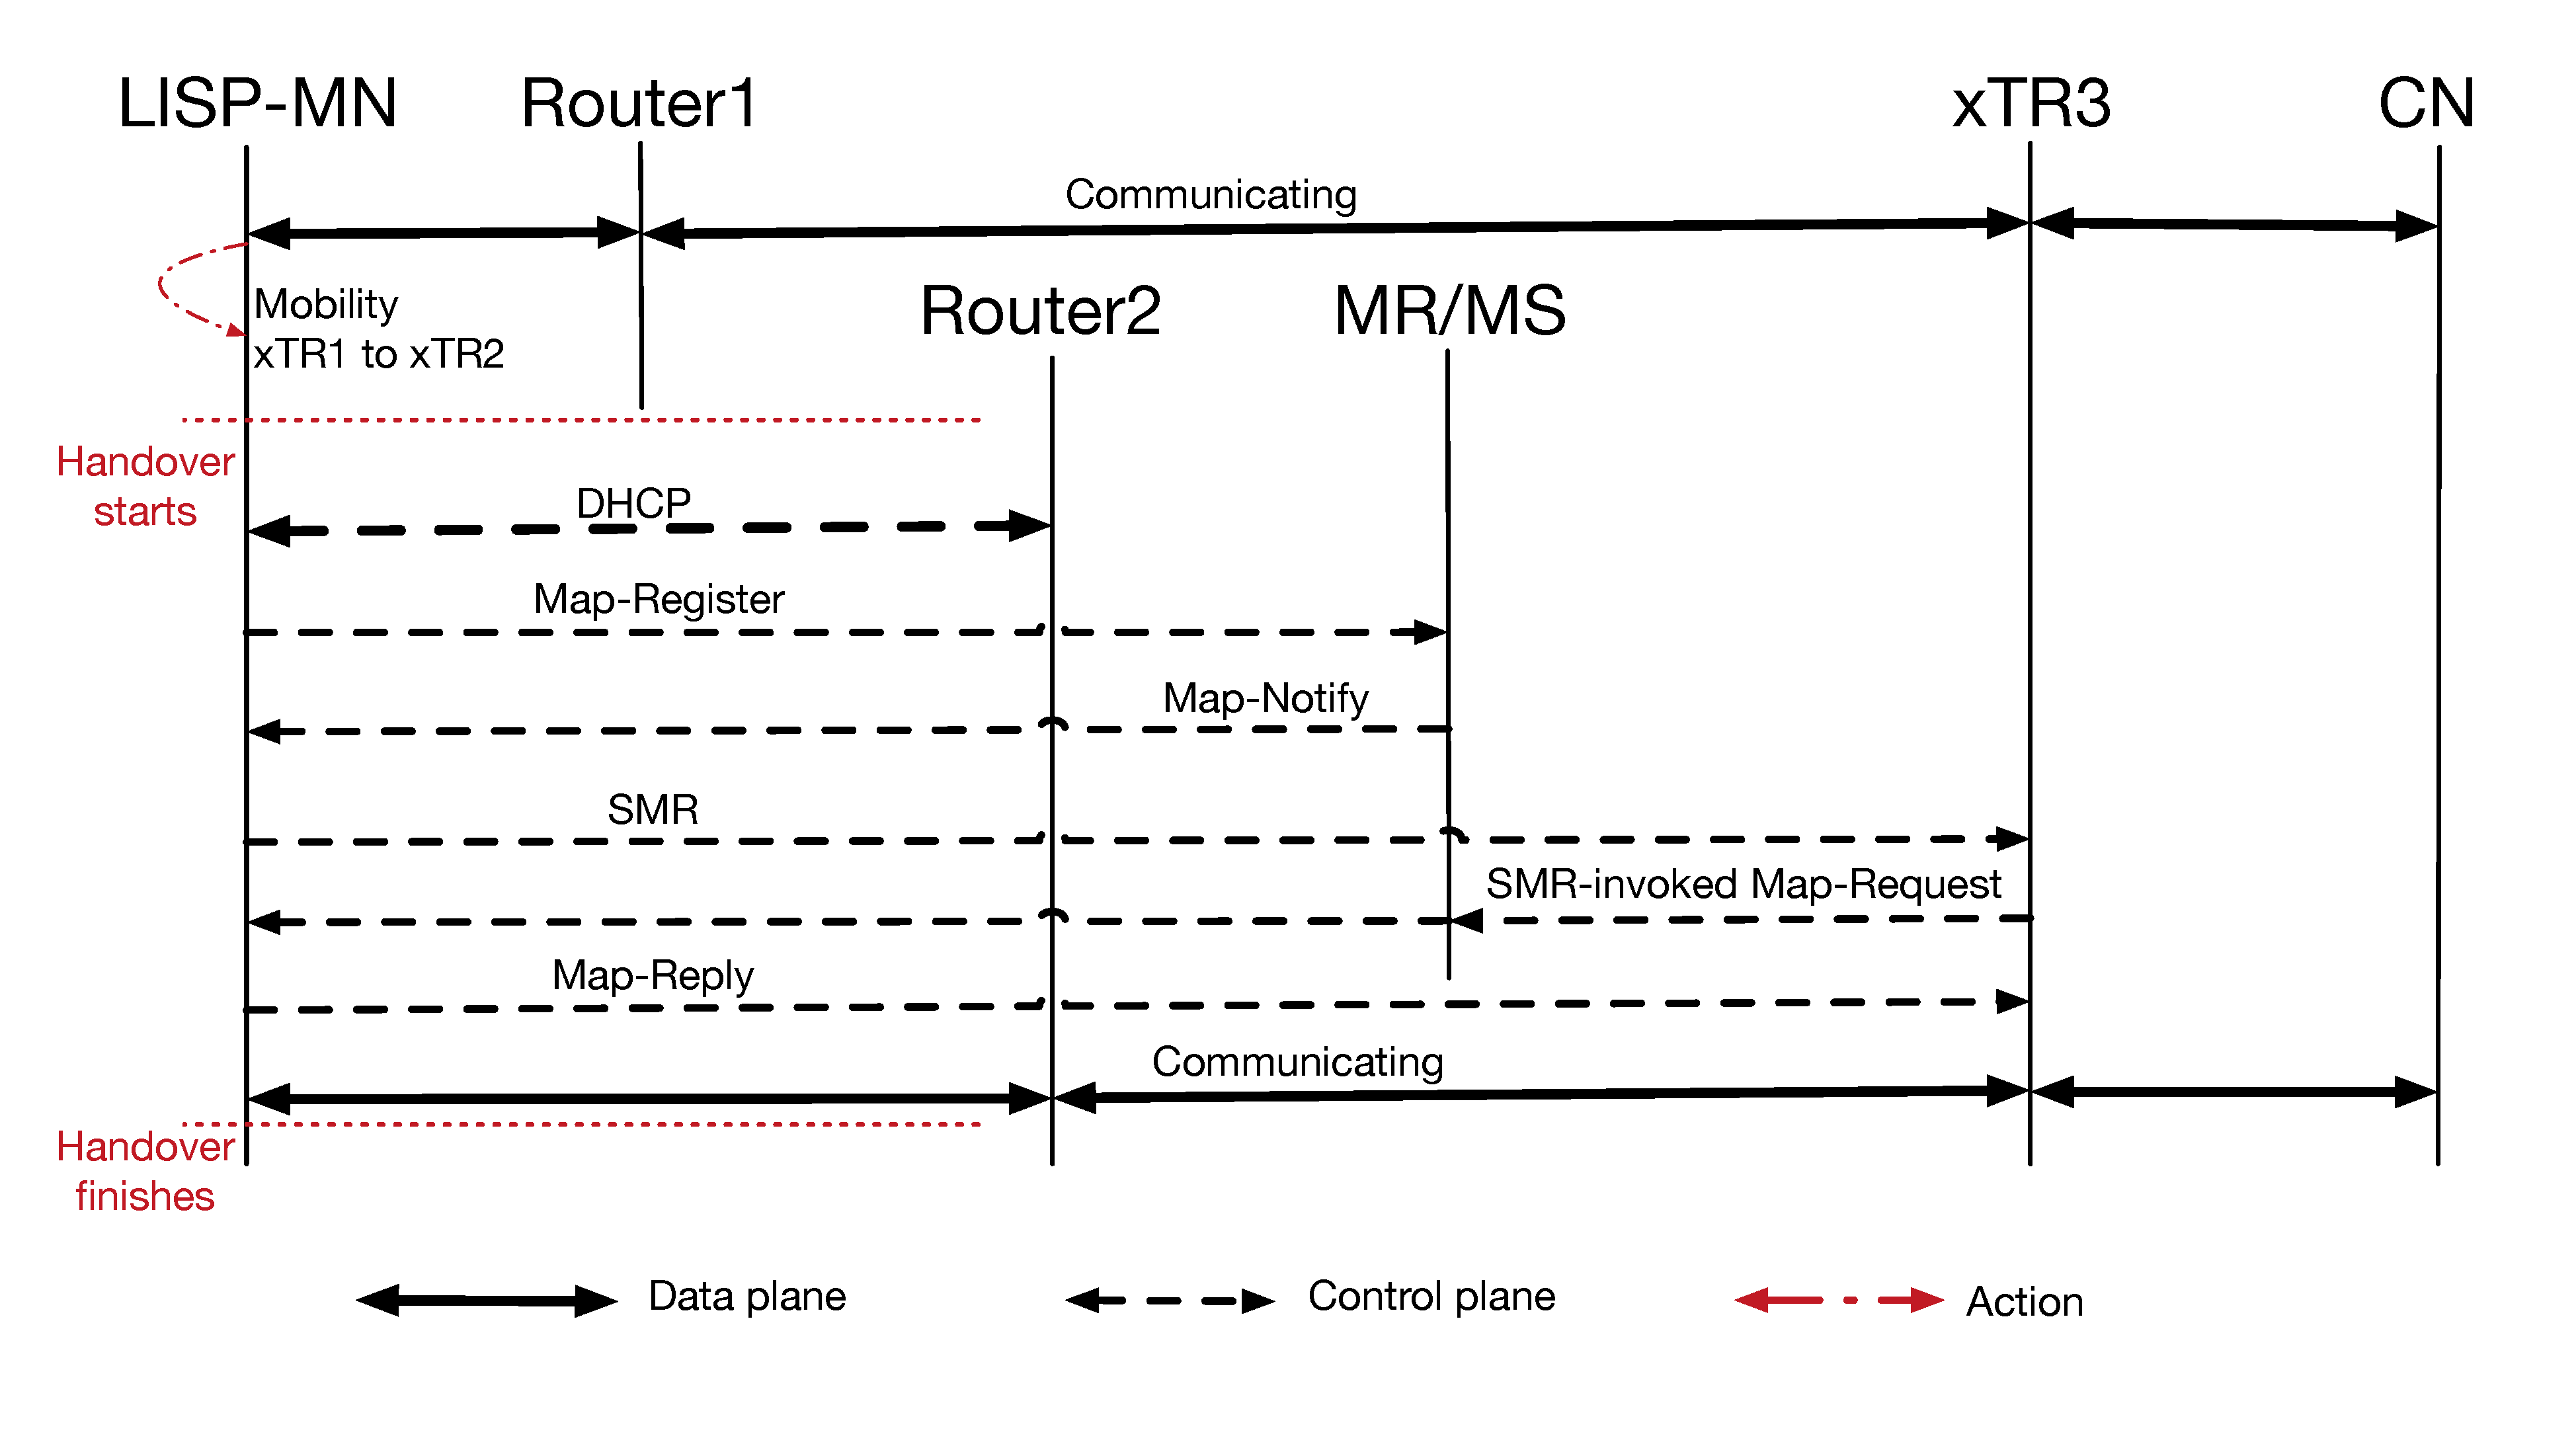
\includegraphics[width=\textwidth]{Pics/Mobility_LISPMN_schema_SMR_simplify}
	\caption{Schema for LISP-MN mobility}
	\label{sim_schema}
\end{figure}
%-< END FIGURE >--------------------------------------------------------------------

The overall handover delay in this paper is defined at the moment that LISP-MN sending DHCP Discover message to xTR\_2 and end up with xTR\_3 receiving the last Map-Reply from xTR\_2. Precisely, it is composed by three parts: the Wi-Fi association delay, the DHCP related delay and LISP SMR delay:
\begin{eqnarray}
	D_{overall} &=& D_{DHCP} + D_{Register} + D_{Notify} + D_{SMR} + D_{invokeSMR} + D_{Reply} \nonumber \\
	&=& D_{DHCP} + 2T_{LISPMN-MDS} + 3T_{LISPMN-xTR_3} \nonumber \\
	&=& D_{DHCP} + 2* (3*2ms) + 3*(3*2ms)\nonumber \\
	&=& D_{DHCP} + 30 ms
\end{eqnarray}
where $D$ is the delay, $BI$ is Beacon Interval, subscriptions $Wi-Fi$, $DHCP$ and $SMR$ respectively refers to Wi-Fi association, DHCP procedure and LISP SMR. (Min value of handover delay = 1.073031 s, where packet sending interval = 0.01 s) 

%-< FIGURE >--------------------------------------------------------------------
\begin{figure}[!th]
	\centering
	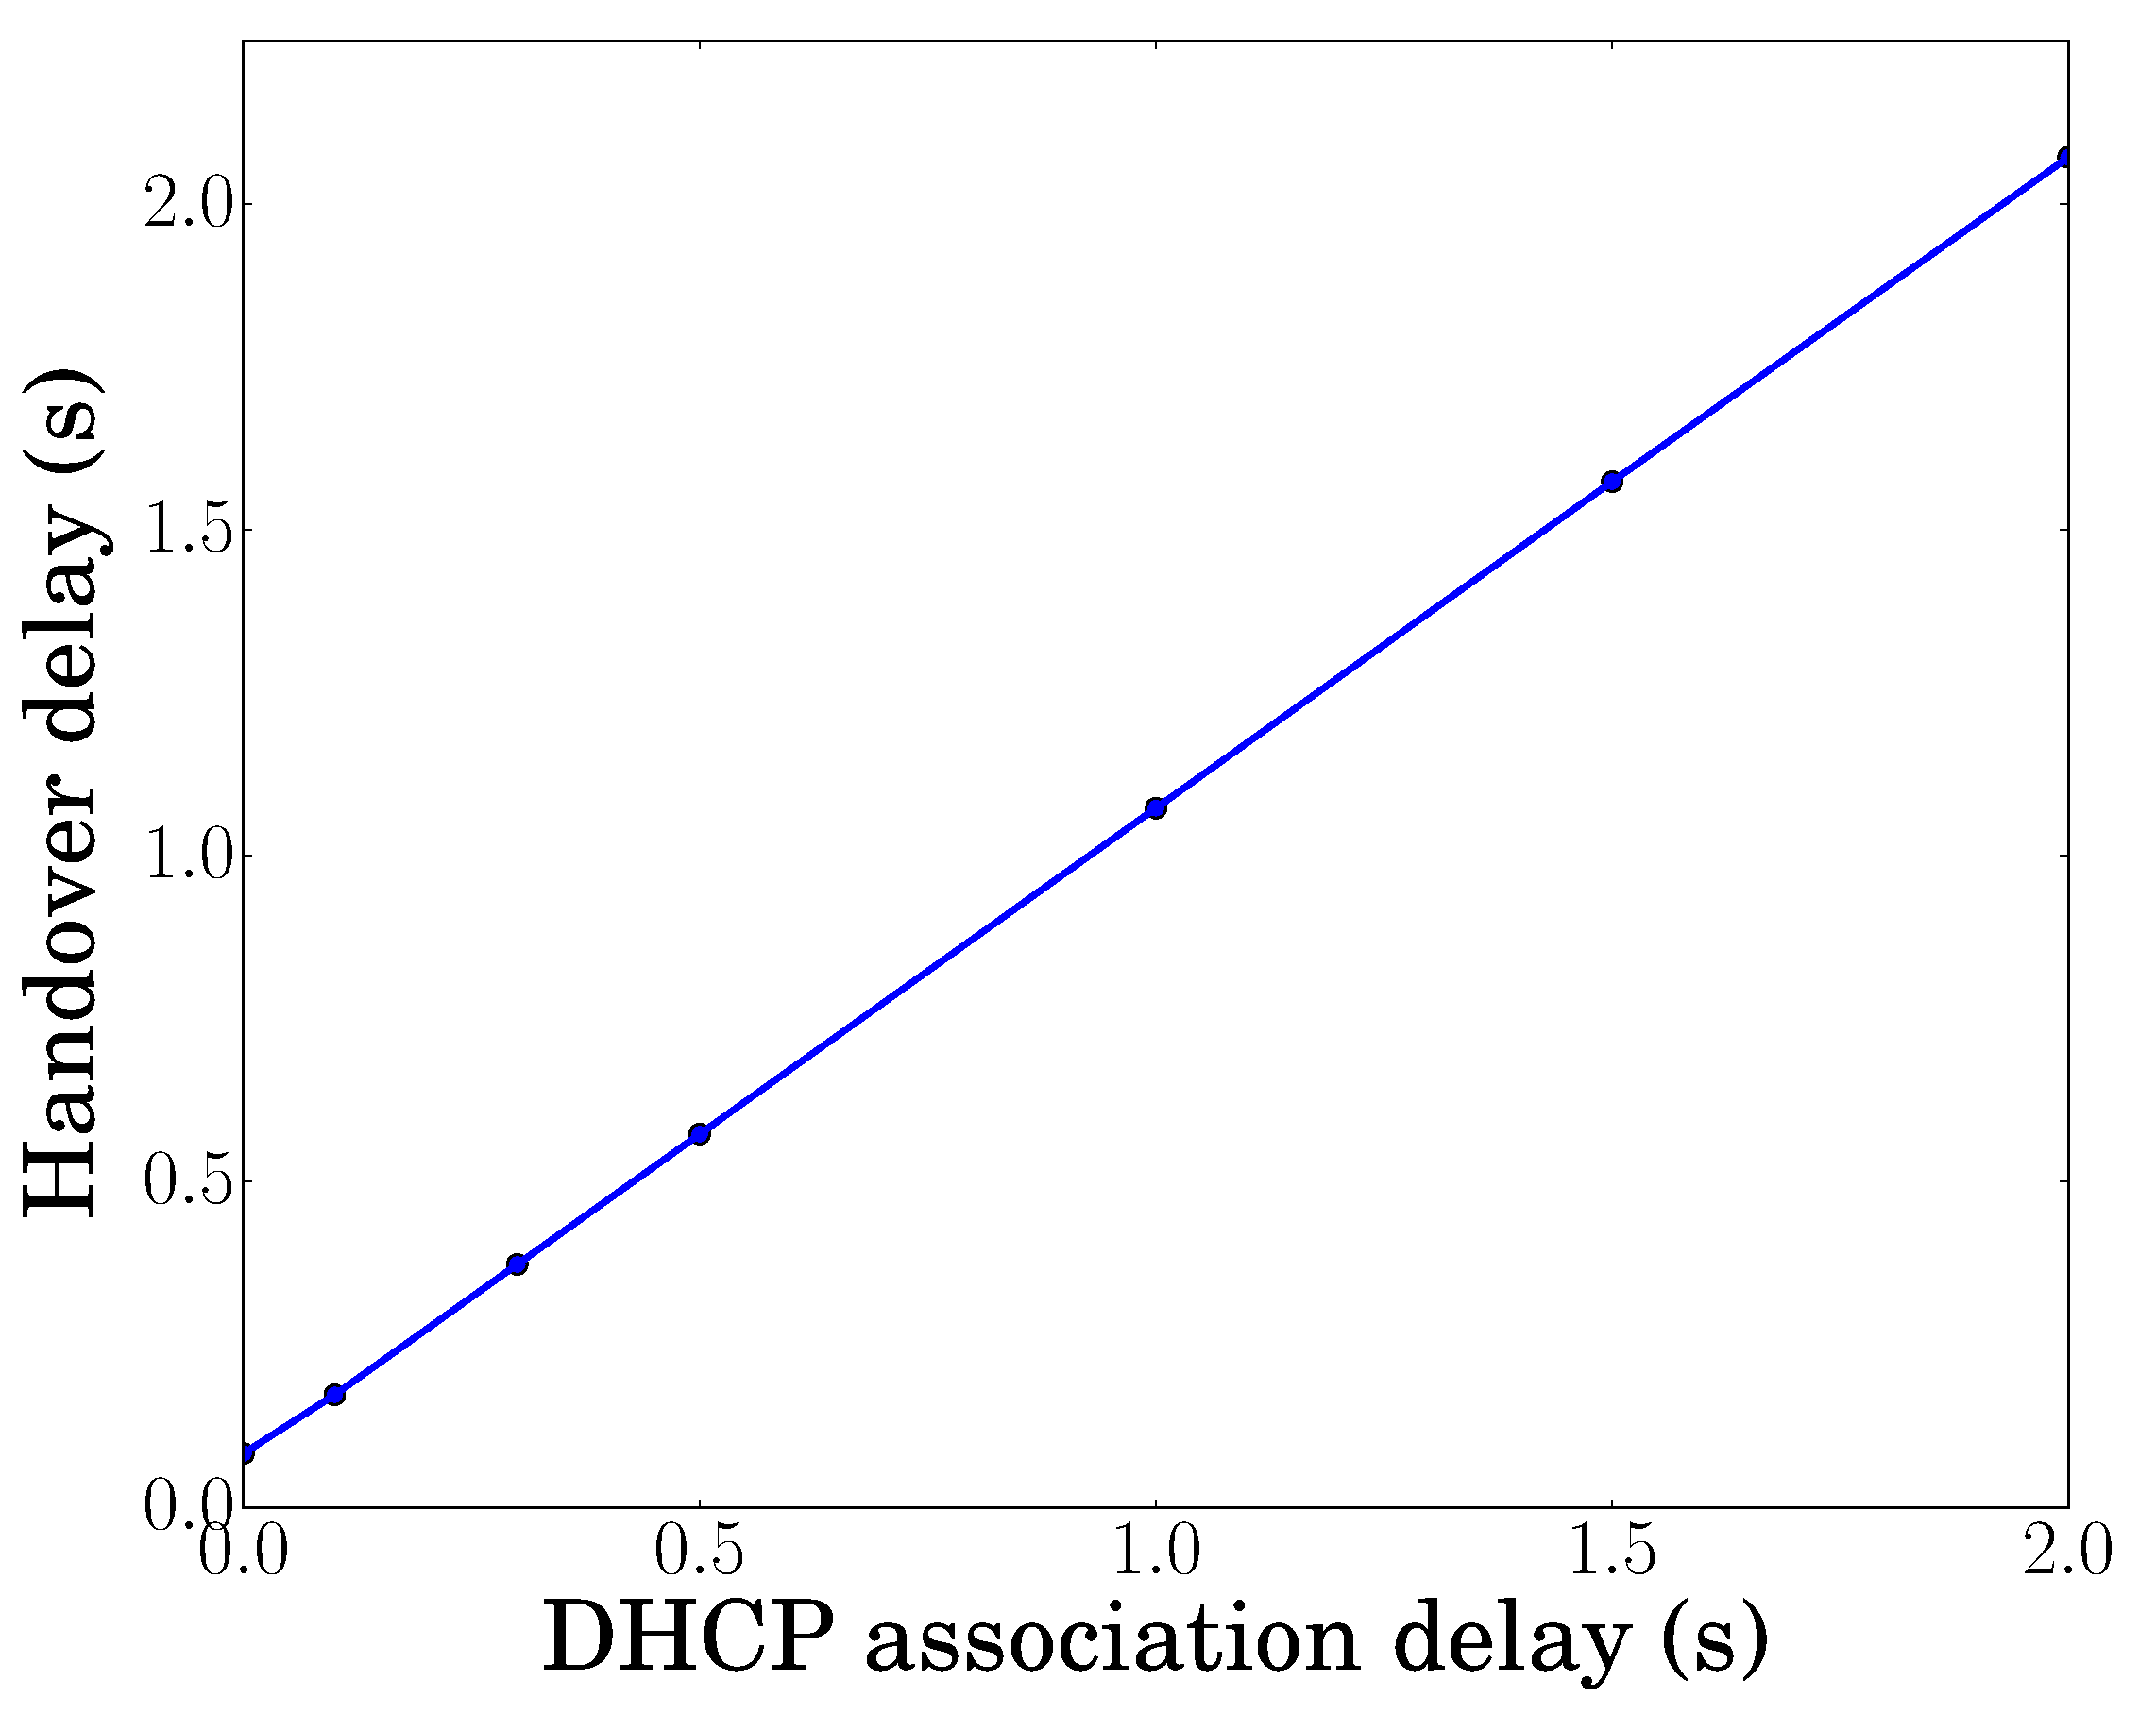
\includegraphics[width=0.7\textwidth]{Pics/LISP_mobility_LISPMN_DHCP}
	\caption{Impact of DHCP association on handover delay}
	\label{LISP_mobility_LISPMN_DHCP}
\end{figure}
%-< END FIGURE >--------------------------------------------------------------------


%-< FIGURE >--------------------------------------------------------------------
\begin{figure}[!th]
	\centering
	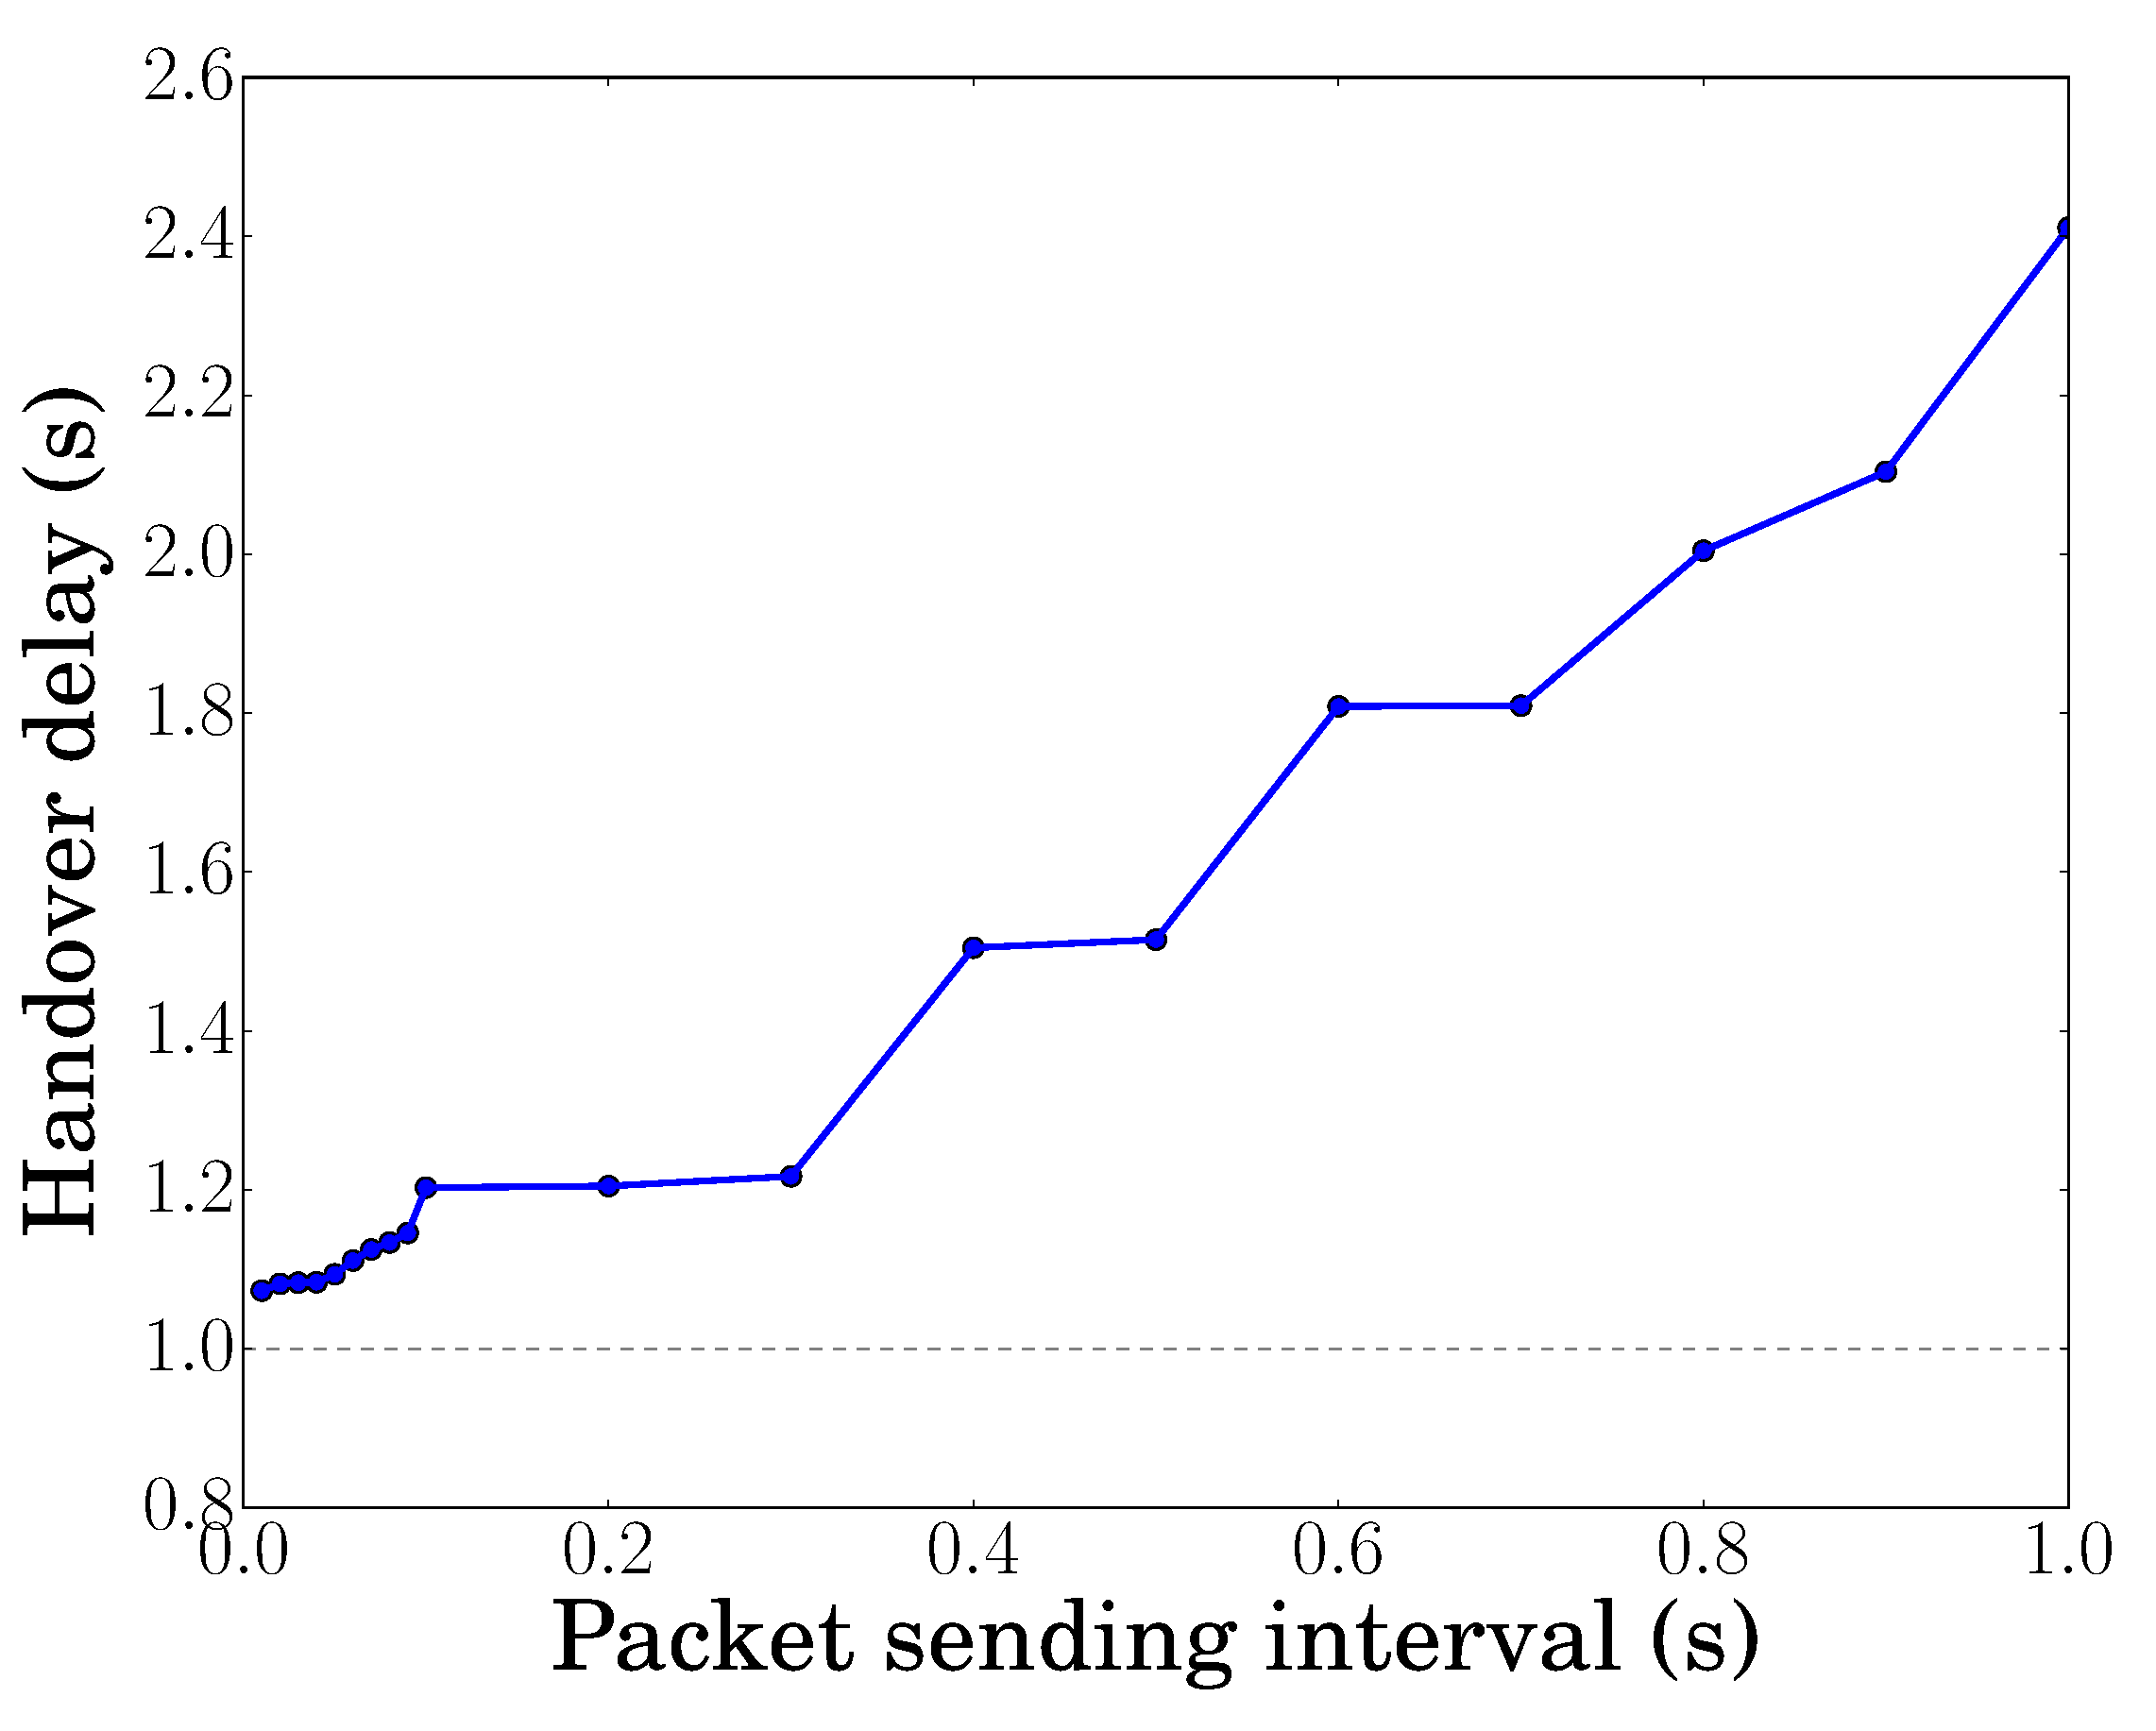
\includegraphics[width=0.7\textwidth]{Pics/LISP_mobility_LISPMN_PacketInterval}
	\caption{Impact of packet sending interval on handover delay}
	\label{LISP_mobility_LISPMN_PacketInterval}
\end{figure}
%-< END FIGURE >--------------------------------------------------------------------


%-< SECTION >--------------------------------------------------------------------
\section{Evaluation for MN in LISP-Site}
\label{sec:ns3_evaluation_xTR}
We validate our LISP/LISP-MN implementation by conducting a simulation and providing a preliminary performance evaluation of handover delay. The simulation topology is shown in Fig.~\ref{sim_scenario}.
%-< FIGURE >--------------------------------------------------------------------
\begin{figure}[!th]
	\centering
	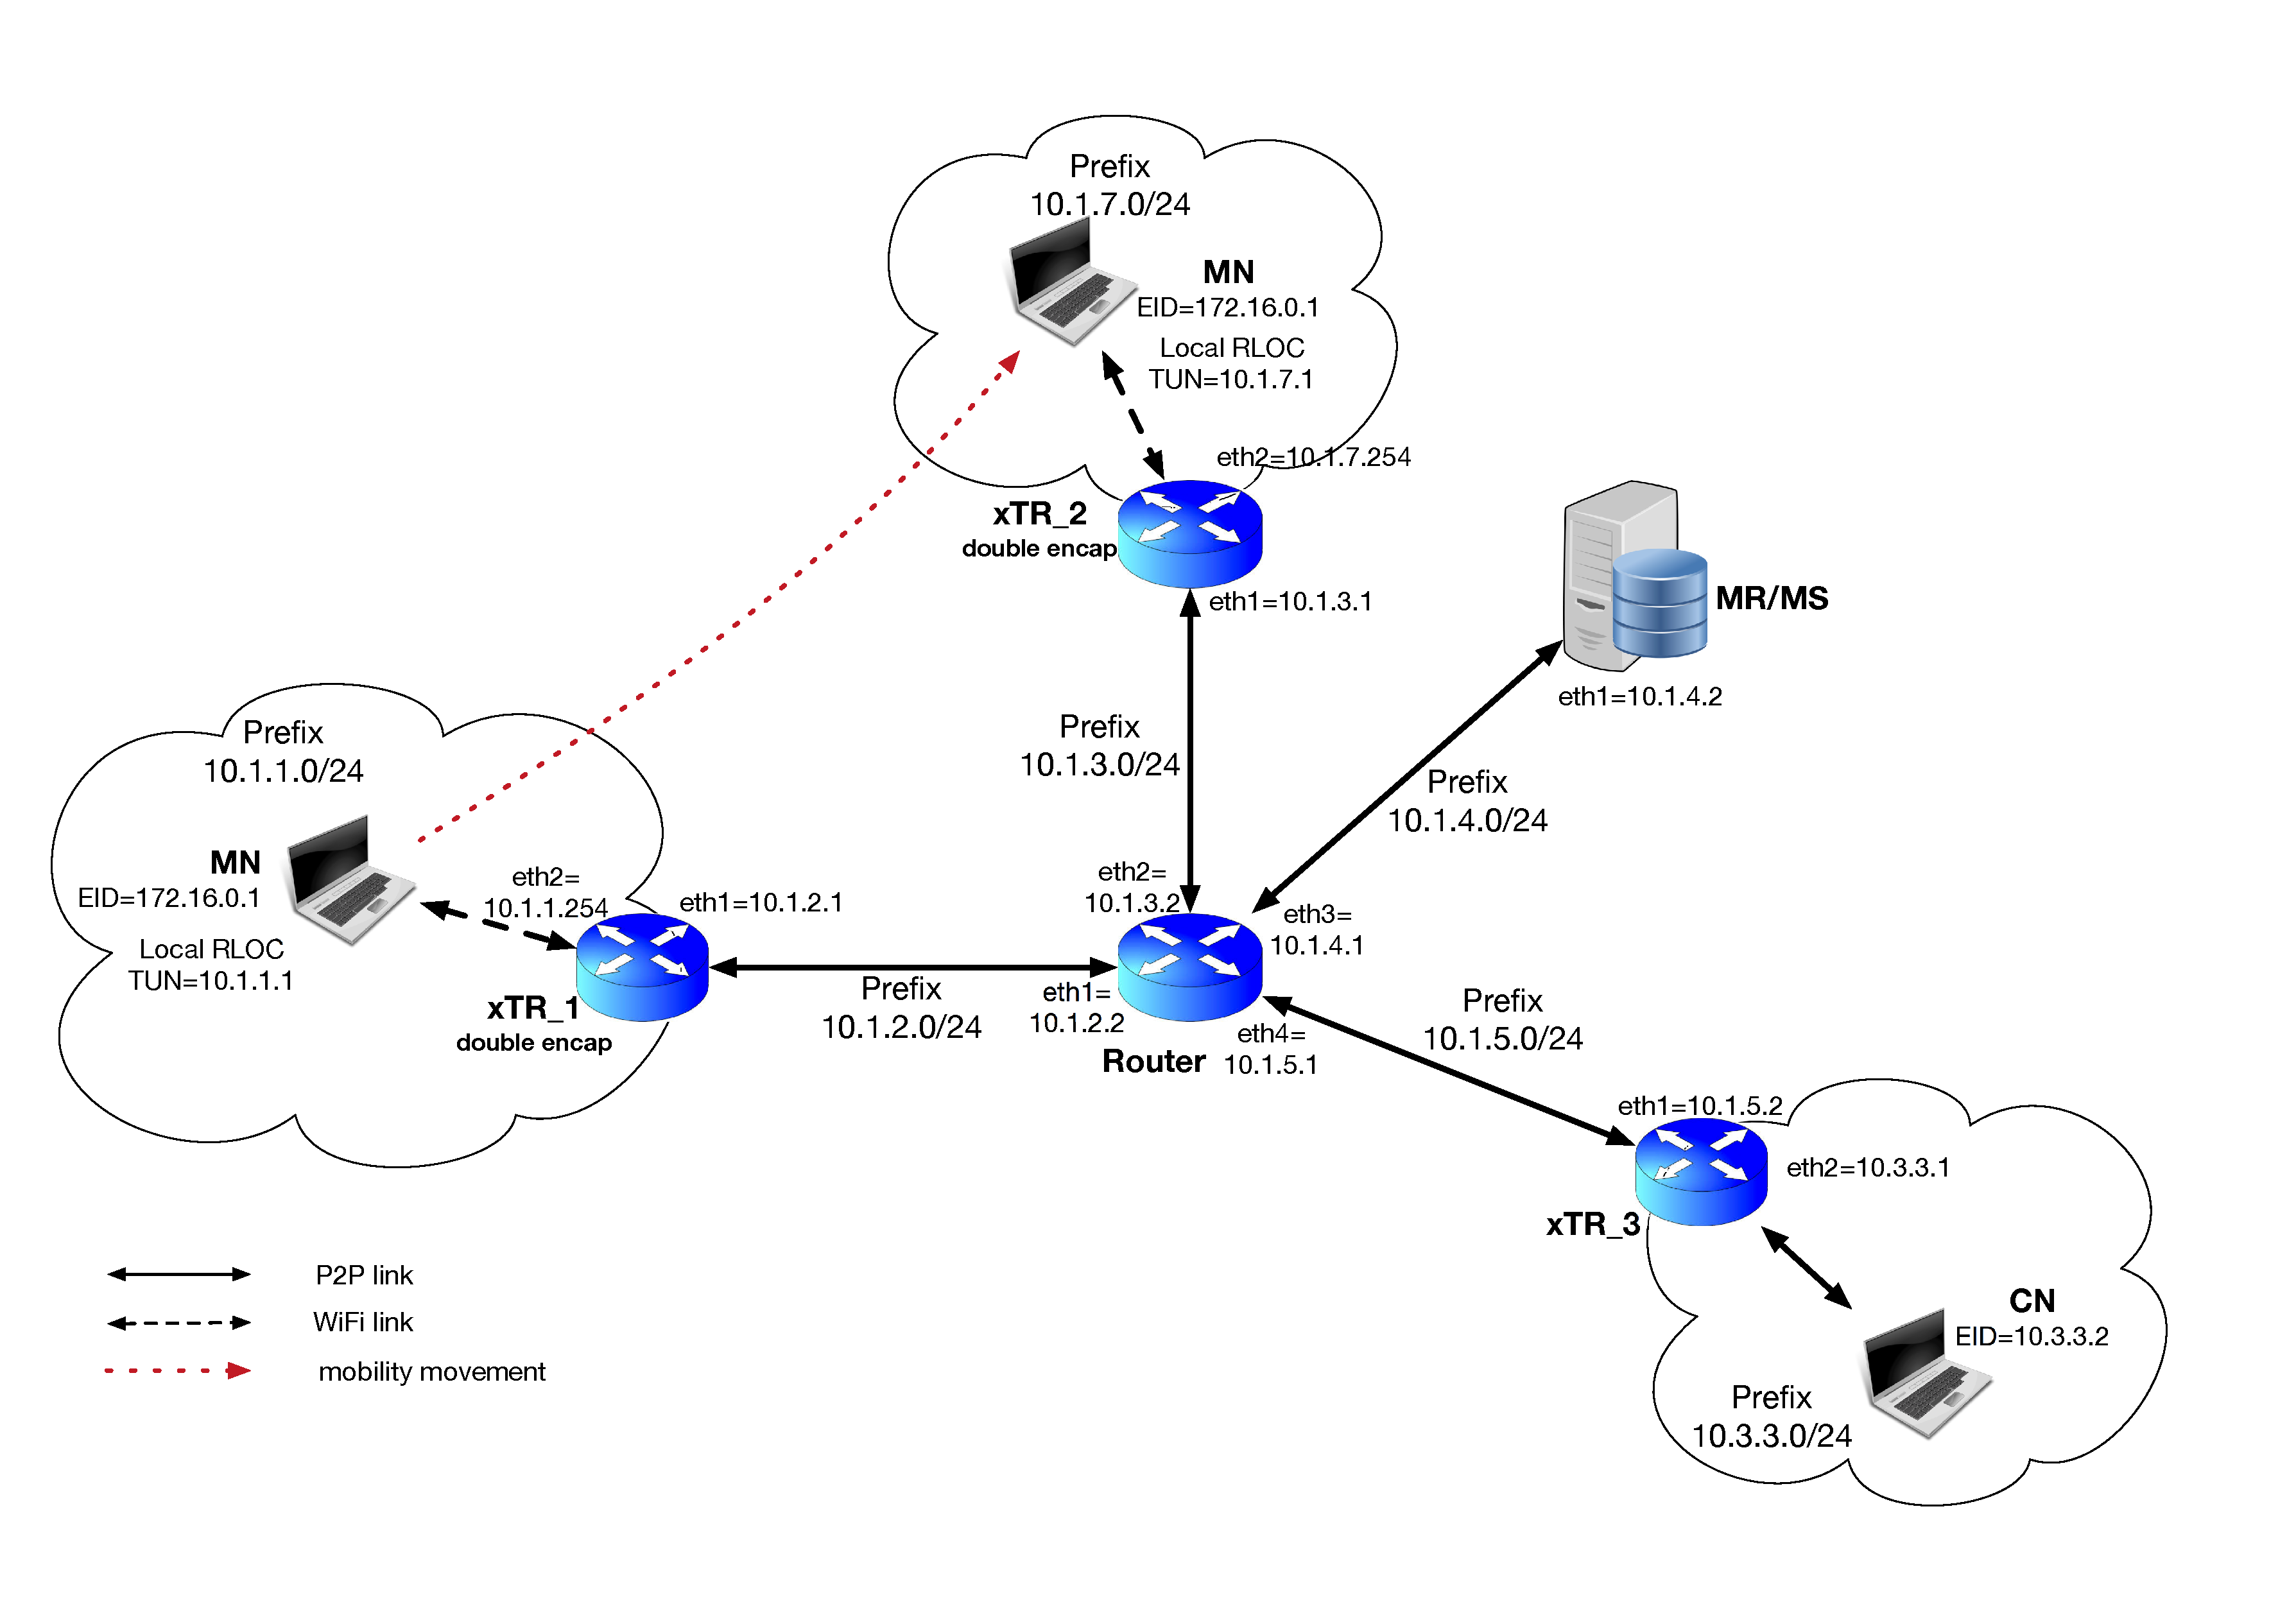
\includegraphics[width=\textwidth]{Pics/mobility_through_subnets_2_encap_topo}
	\caption{LISP mobility simulation scenario for double encapsulation}
	\label{sim_scenario}
\end{figure}
%-< END FIGURE >--------------------------------------------------------------------

%-< SUB SECTION >--------------------------------------------------------------------
\subsection{Simulation Setup}
\label{subsec:ns3_setup_xTR}
%\begin{itemize}
%    \item Topology of simulation setup
%    \item The simulation parameter settings
%\end{itemize}
In our simulation, a LISP-MN with permanent EID 172.16.0.1 is initially placed in network 10.1.1.0/24. An \emph{echo} application on LISP-MN sends one packet per second to a remote stationary node CN with EID 10.3.3.2, and the LISP-MN moves into network 10.1.7.0/24 at speed of $7.07m/s$. The distance between xTR\_1 and xTR\_2 is $170m$. LISP-MN node uses Wi-Fi to connect to xTR\_1. At a certain moment during the moving, the Wi-Fi link between LISP-MN and xTR\_1 is down, which triggers the handover procedure. Afterwards, LISP-MN connects to xTR\_2 and reestablishes the communication with CN node. The total simulation time is set to $45s$ and the DHCP procedure delay is set to $1s$. We conduct many times of simulations with the various beacon interval of Wi-Fi channel in the range of $0.05s$ to $2s$.

%-< SUB SECTION >--------------------------------------------------------------------
\subsection{Results}
\label{sec:ns3_results_xTR}

%-< FIGURE >--------------------------------------------------------------------
\begin{figure}[!th]
	\centering
	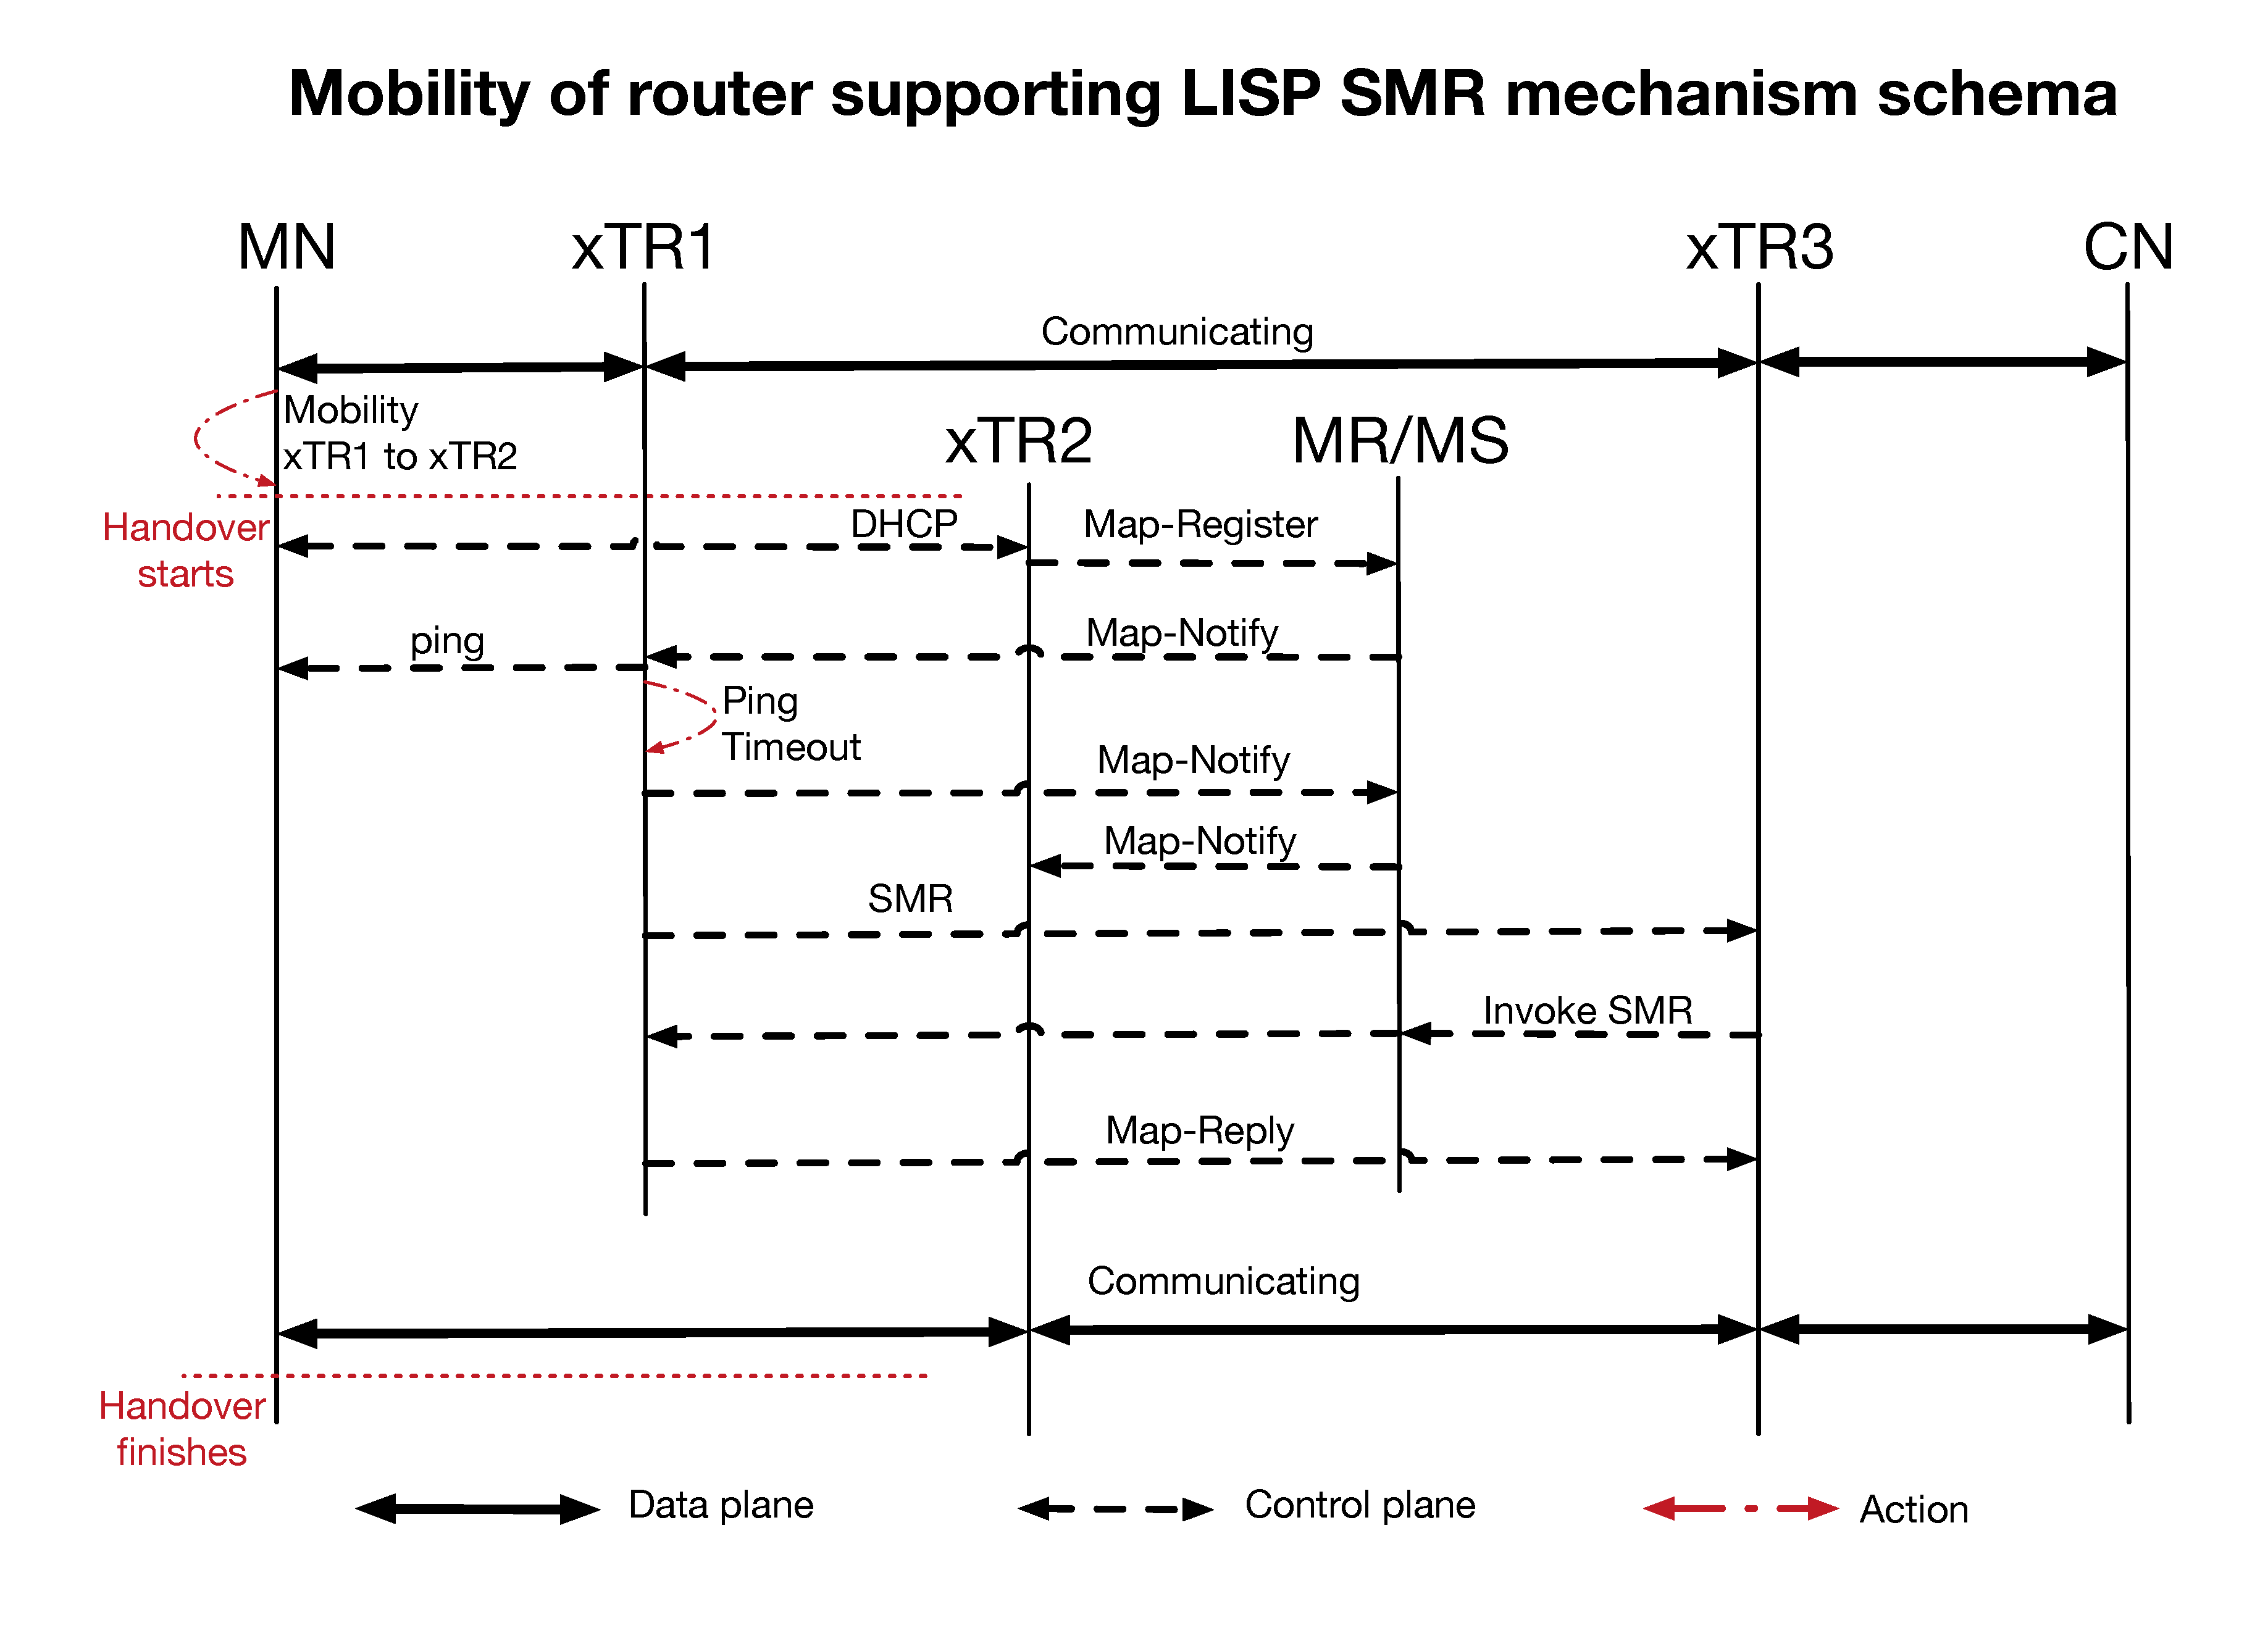
\includegraphics[width=\textwidth]{Pics/Mobility_xTR_schema_SMR_simplify}
	\caption{Schema for LISP-MN mobility}
	\label{sim_schema}
\end{figure}
%-< END FIGURE >--------------------------------------------------------------------

The overall handover delay in this paper is defined at the moment that LISP-MN sending DHCP Discover message to xTR\_2 and end up with xTR\_3 receiving the last Map-Reply from xTR\_2. Precisely, it is composed by three parts: the Wi-Fi association delay, the DHCP related delay and LISP SMR delay:
\begin{eqnarray}
D_{overall} &=& D_{DHCP} + D_{Register} + D_{Notify} + D_{SMR} + D_{invokeSMR} + D_{Reply} \nonumber \\
&=& T_{xTR_2-MDS} + T_{MDS-xTR_1} + D_{DHCP} + 3T_{xTR_2-xTR_3} \nonumber \\
&=& 2* (2*2ms) + D_{DHCP} + 3*(2*2ms) \nonumber \\
&=& D_{DHCP} + 20 ms
\end{eqnarray}
where $D$ is the delay, $BI$ is Beacon Interval, subscriptions $Wi-Fi$, $DHCP$ and $SMR$ respectively refers to Wi-Fi association, DHCP procedure and LISP SMR. $CheckAlive$ is the delay that xTR\_1 checks if MN still connects to it. For example, xTR\_1 can simply \emph{ping} MN. If MN still connects to it, it will reply to mapping system that itself is still RLOC of MN. Otherwise, if \emph{ping} meets timeout, xTR\_1 will tell the mapping system that MN has left, and sends SMR to the CNs in its cache. The later situation has higher delay, because xTR\_1 needs to wait until timeout of \emph{ping}. (Min value of simulation = 1.067679 s, where includes 1 s of DHCP delay)

%-< FIGURE >--------------------------------------------------------------------
\begin{figure}[!th]
	\centering
	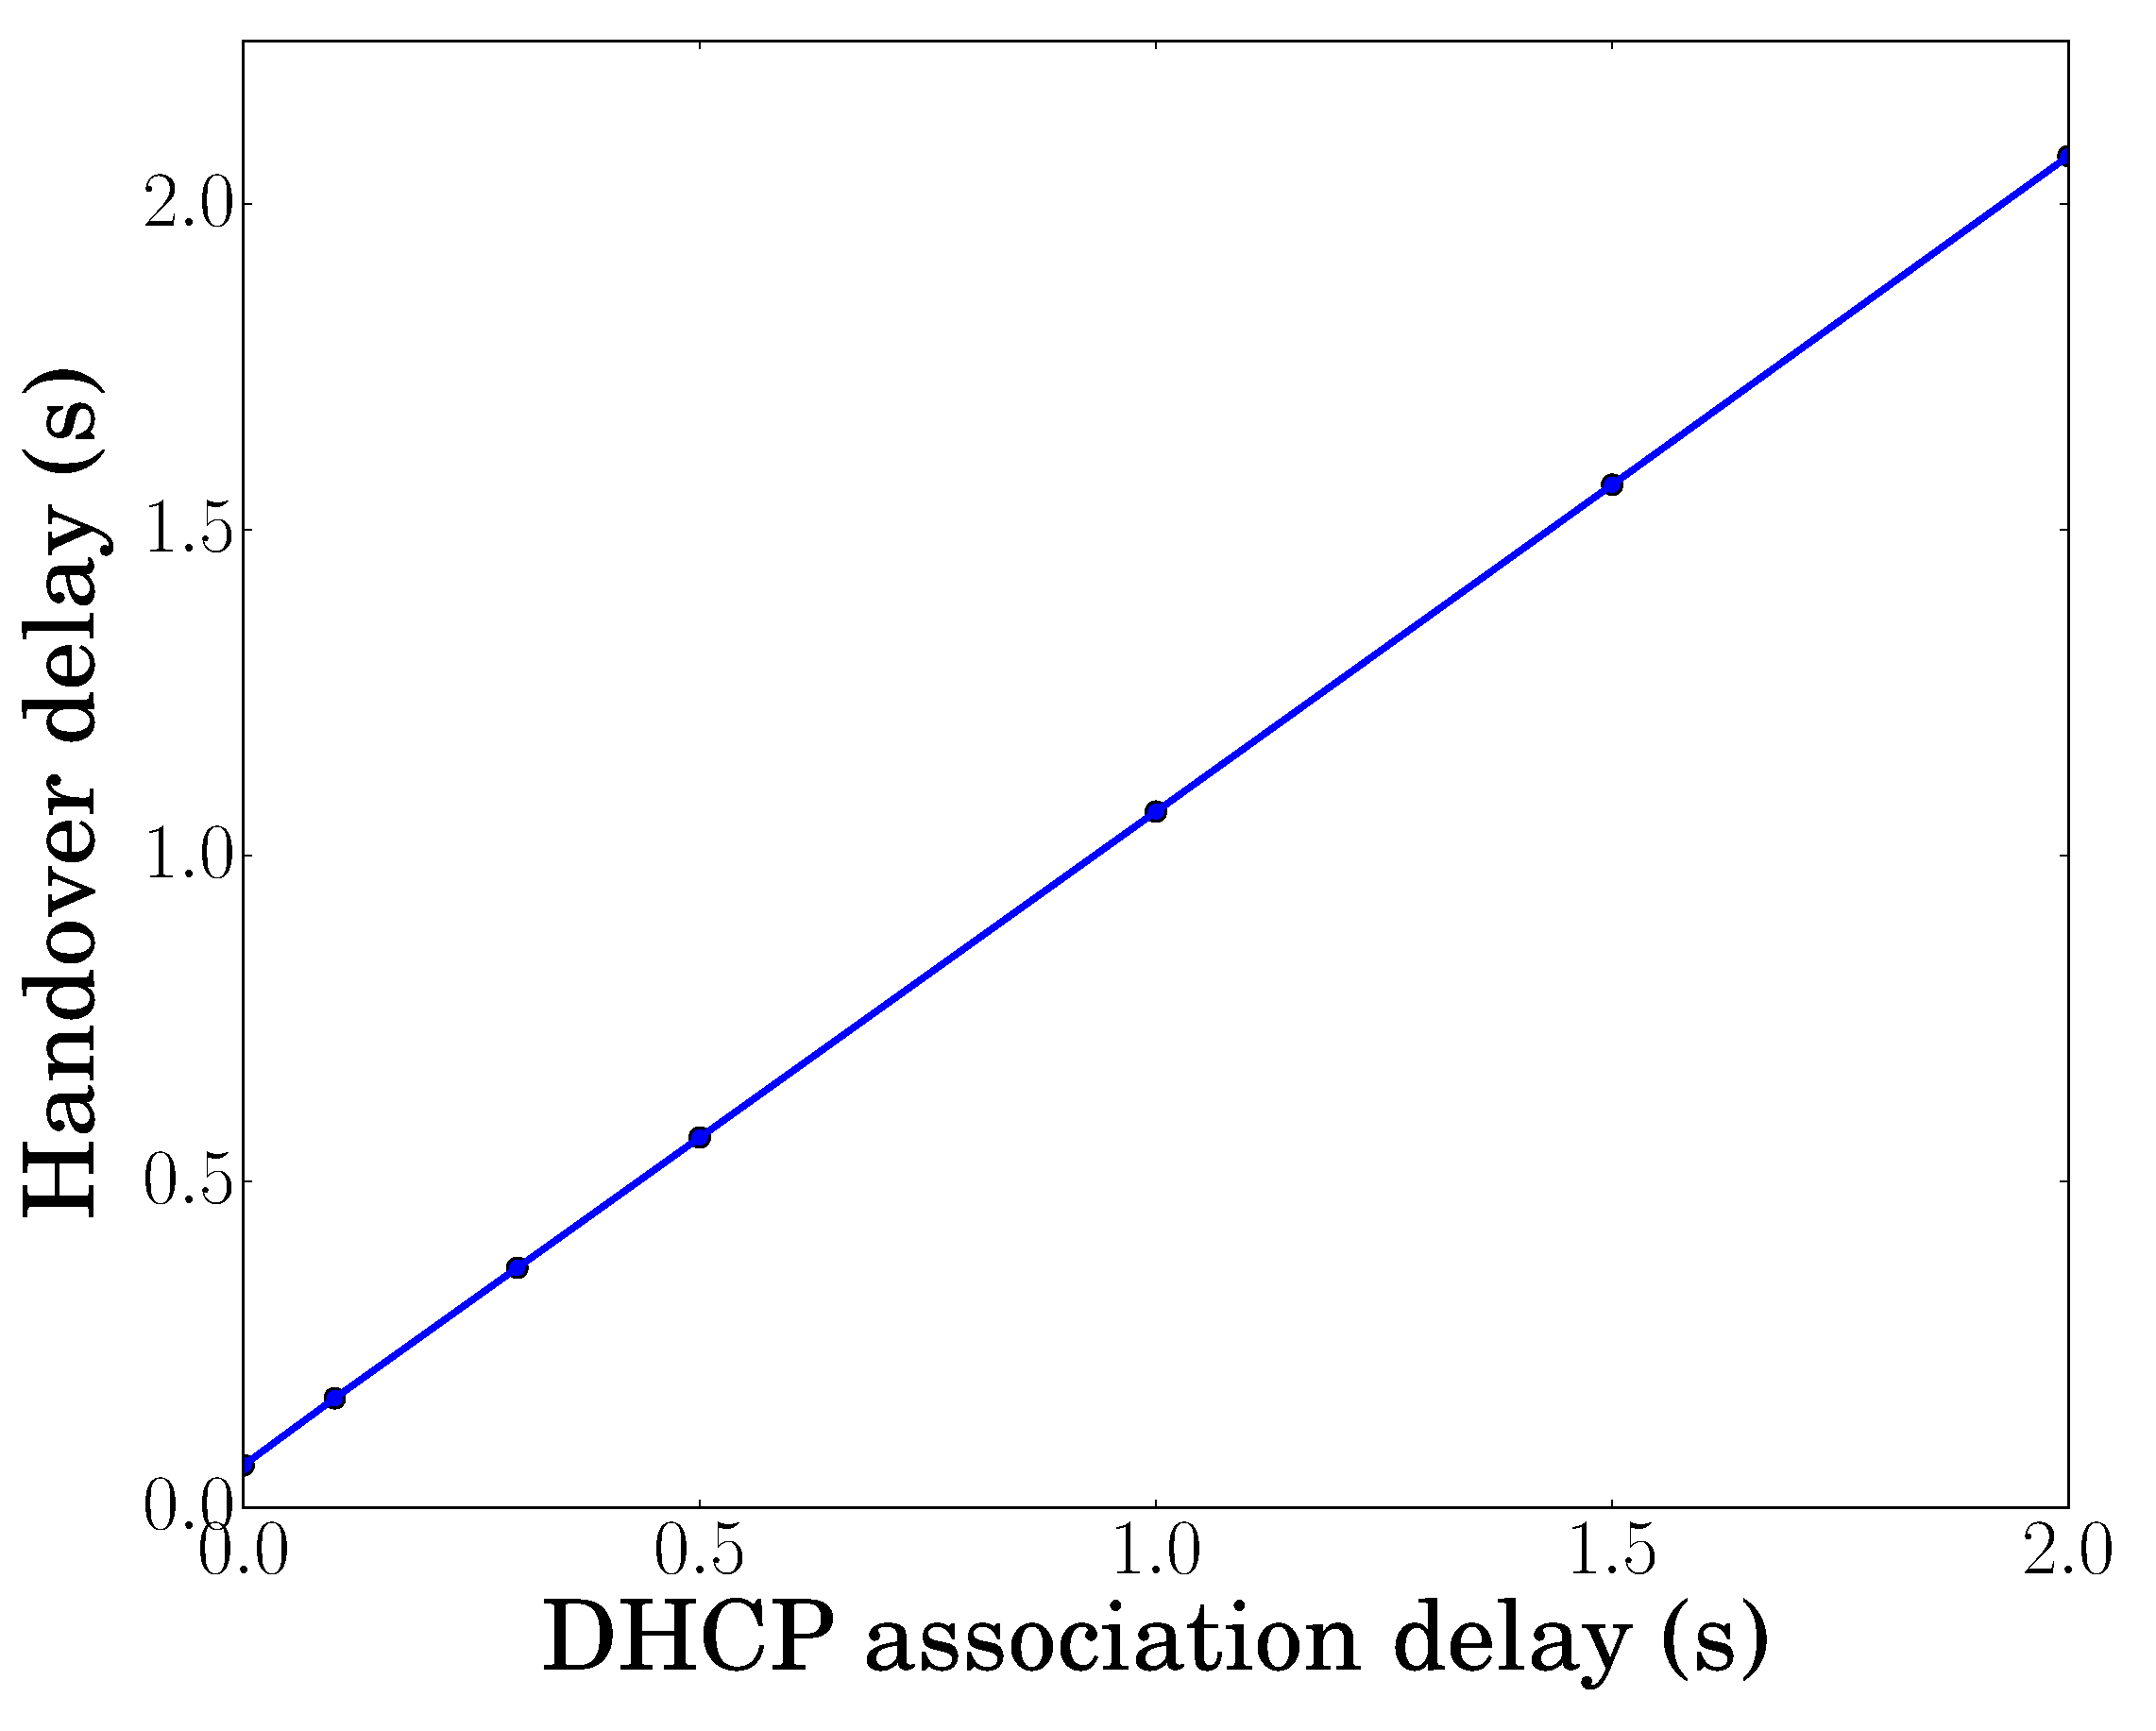
\includegraphics[width=0.7\textwidth]{Pics/LISP_mobility_xTR_DHCP}
	\caption{Impact of DHCP association on handover delay}
	\label{LISP_mobility_xTR_DHCP}
\end{figure}
%-< END FIGURE >--------------------------------------------------------------------


%-< FIGURE >--------------------------------------------------------------------
\begin{figure}[!th]
	\centering
	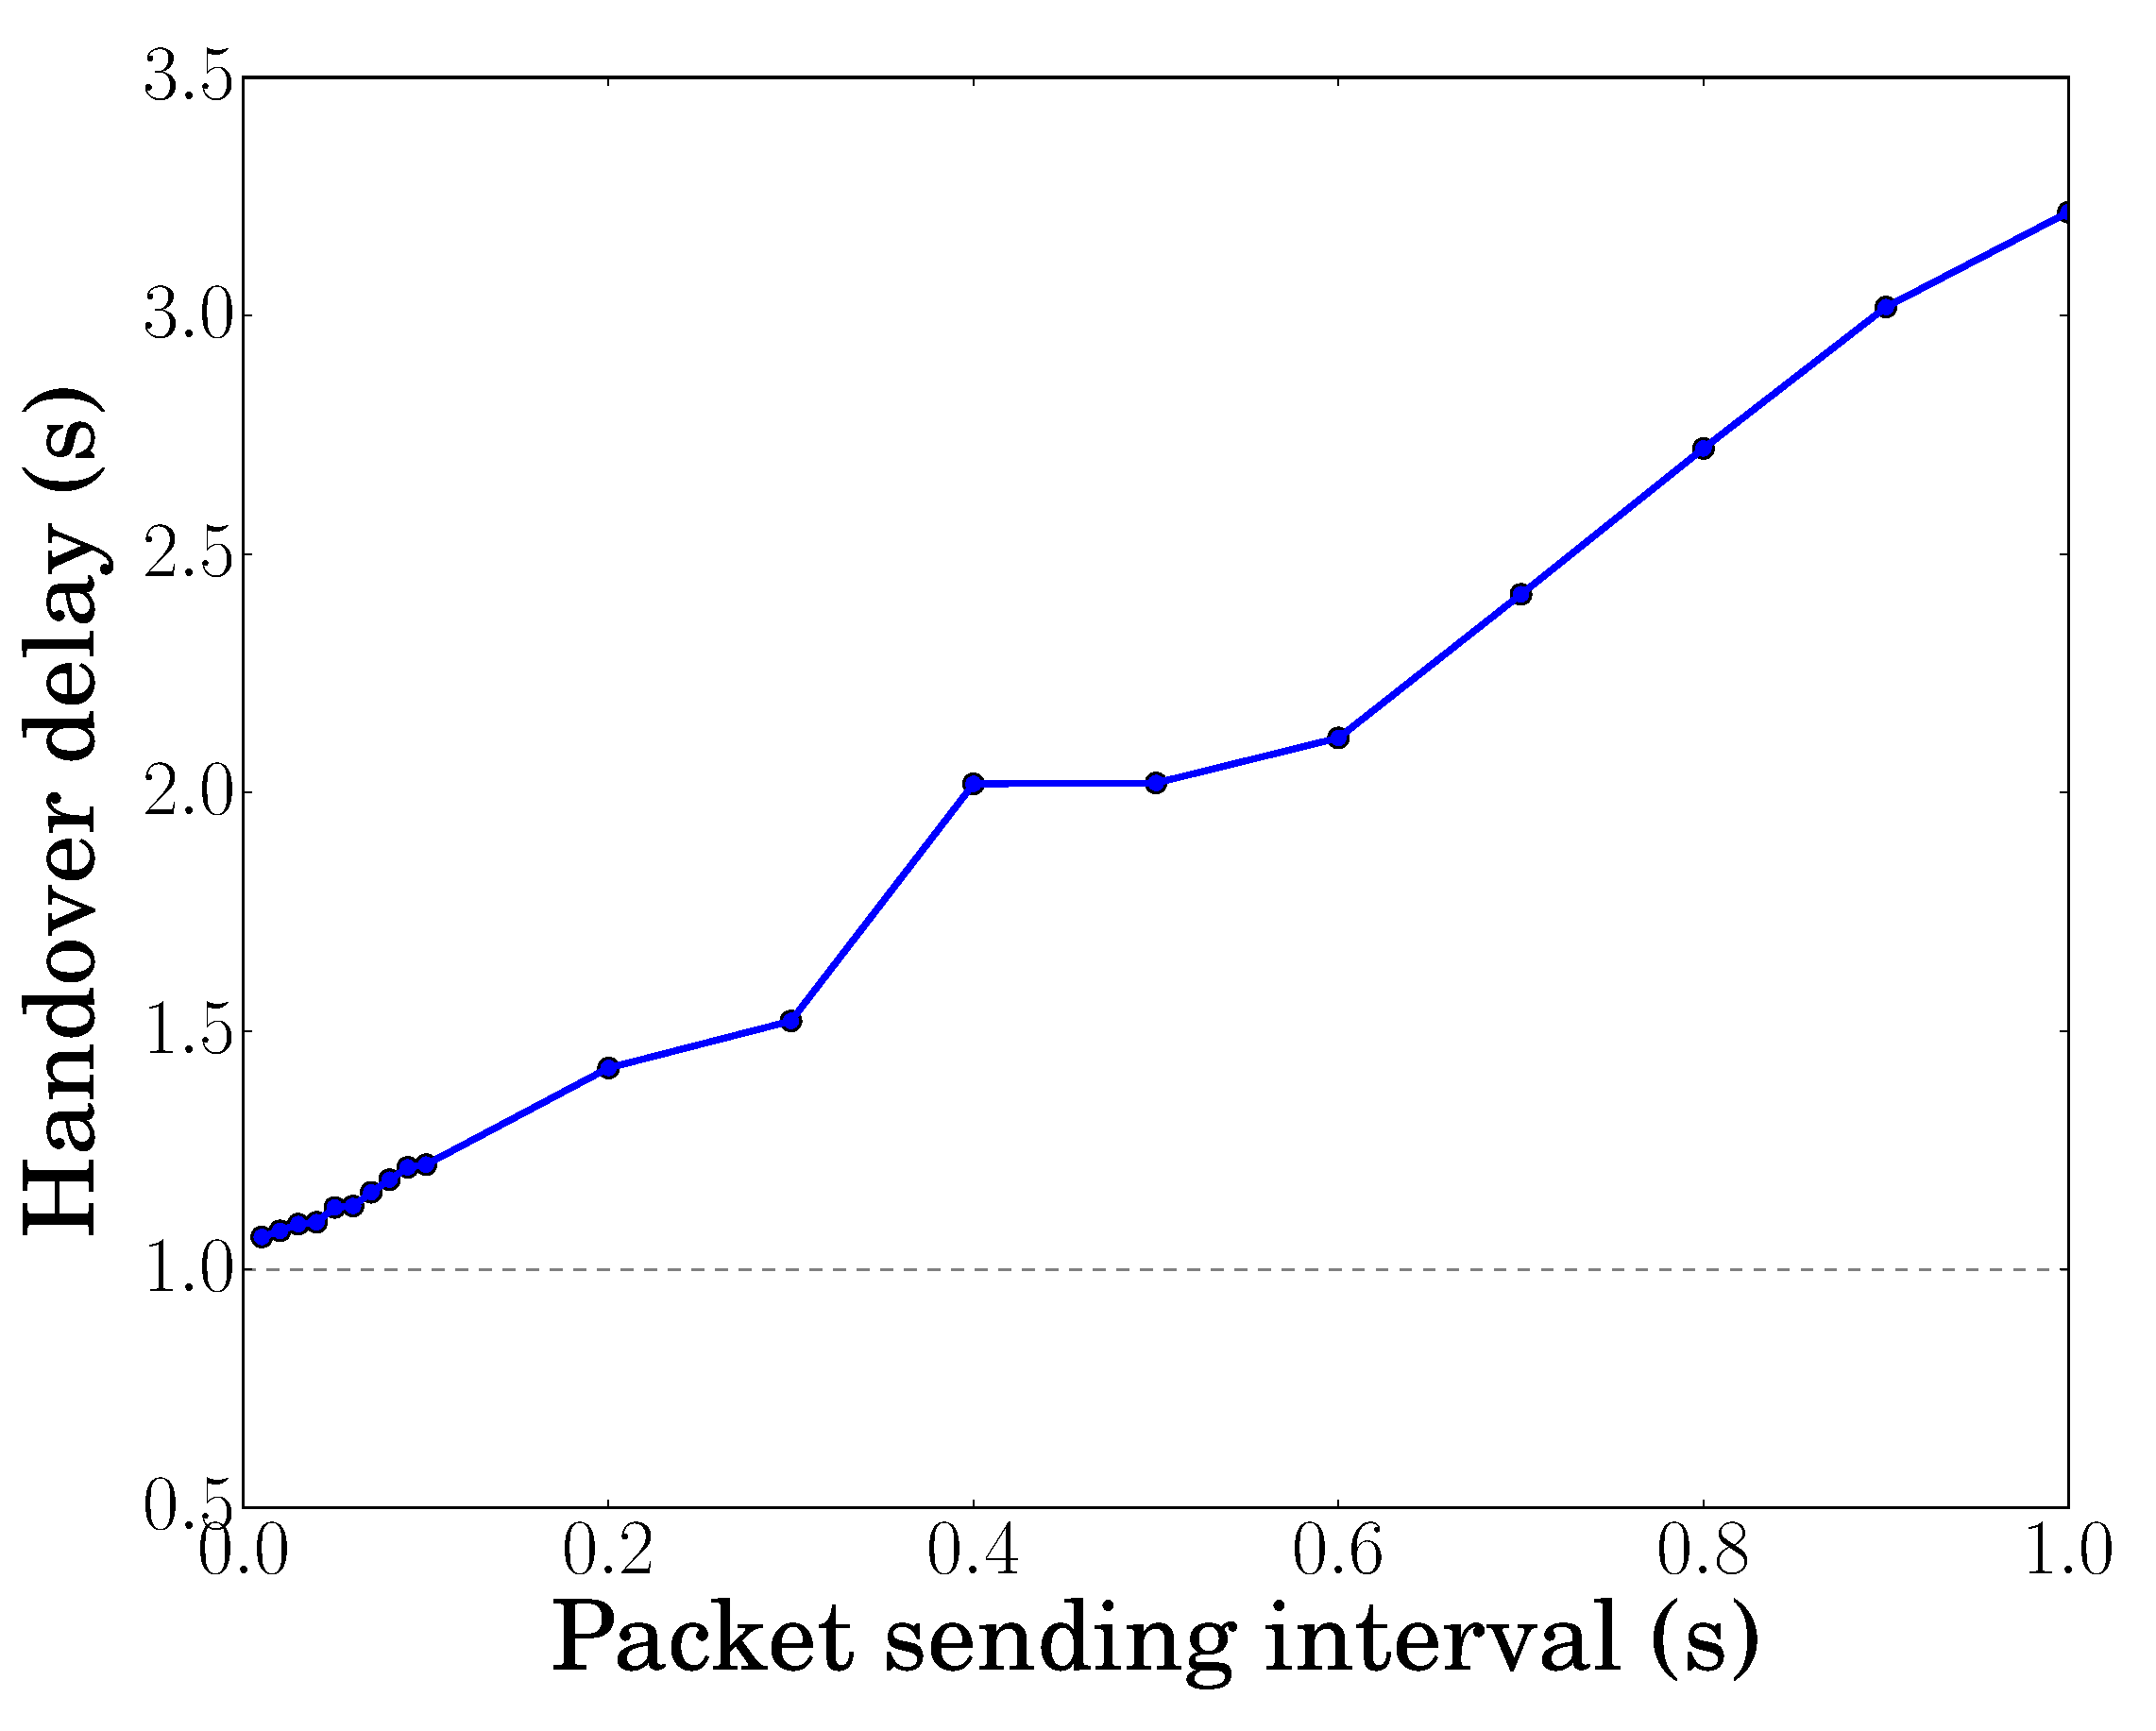
\includegraphics[width=0.7\textwidth]{Pics/LISP_mobility_xTR_PacketInterval}
	\caption{Impact of packet sending interval on handover delay}
	\label{LISP_mobility_xTR_PacketInterval}
\end{figure}
%-< END FIGURE >--------------------------------------------------------------------

%-< SECTION >--------------------------------------------------------------------
\section{Conclusion}
\label{sec:ns3_conclusion}
%\begin{itemize}
%    \item The validation of the implemented simulator
%    \item LISP-MN handover analysis
%    \item The potential of the implemented simulator
%\end{itemize}
As a promising technology for the future Internet architecture, LISP attracts more and more attention. There exist some LISP implementations, but they do not support LISP-MN or they are proprietary. Further, although measurements on LISP-testbeds can provide real time performance, due to the complicated topological structure, it is somewhat like a black box test which hinders us to find the exact explanation for some results. This highlights the importance to have an open source simulator for LISP in particular to support LISP-MN functionality. In this paper, we present our implementation for LISP/LISP-MN within ns-3, since the latter is a largely accepted simulator in networking research. The simulation results show that our implementation works well, and reveal the current LISP-MN proposal with a double encapsulation that has an high level delay during handover procedure. Our simulator can be a perfect choice to test the improvements of LISP-MN.

There are two possible directions to support IP mobility in LISP: host-based (i.e. LISP-MN) and network-based (i.e., xTR) mobility. We can compare the performance between LISP double encapsulation described in this paper with only host supporting LISP and only router supporting LISP leveraging our proposed simulator. As Map-Versioning~\cite{rfc6834} is another Mapping Cache update mechanism, we can also compare the performance between it and SMR that we present in this paper by our simulator.
